\chapter{Model-based Reinforcement Learning}
\label{chap4}
\textit{This chapter comprehensively examines the application of data-driven methods to implement \ac{MBRL} for optimal gait control in soft quadruped robots, while also presenting the robot's control architecture.}

\section{Method of Modelling in MBRL}
\subsection{Notation}
The goal of reinforcement learning is to learn a policy that maximizes the cumulative rewards obtained over a sequence of time steps. At each discrete time step denoted by $t$, an agent interacts with its environment. The agent finds itself in a specific state $\mathbf{s}_t$ belonging to the state space $\mathcal{S}$, then performs an action $\mathbf{a}_t$ from the set of possible actions $\mathcal{A}$. Following the action, the agent receives an associated reward $r_t$, which depends on the chosen state and action. Afterward, the agent transitions to a new state $\mathbf{s}_{t+1}$ in a discrete time system. These transitions are determined by the underlying, yet unknown, dynamics function $f$, defined as a mapping from pairs of states and actions to subsequent states $f: (\mathbf{s}_t, \mathbf{a}_t) \rightarrow \mathbf{s}_{t+\Delta t}$. 

In the context of \ac{MBRL}, a surrogate model is developed to approximate the dynamics of the environment. This model is employed to predict the future outcomes of actions and states, aiding the agent in making informed decisions. The learned dynamics function is denoted as $\hat{f}_\theta(\mathbf{s}_t, \mathbf{a}_t)$, and it is parameterized by $\theta$. This learned function accepts the current state $\mathbf{s}_t$ and the action $\mathbf{a}_t$ as inputs and produces an estimate of the future state $\mathbf{s}_{t+1}$ that the agent will encounter after taking the specified action. The parameter $\theta$ captures the characteristics of the learned function, determining its behavior. In this thesis, the chosen approach involves representing the learned dynamics function $\hat{f}_\theta(\mathbf{s}_t, \mathbf{a}_t)$ using a deep neural network. This neural network is designed to capture intricate relationships between the input state and action, allowing it to approximate the complex and often nonlinear dynamics of the environment. 

Before initiating the training process, a dataset $\mathcal{D}$ was assembled through the collection of training samples. These samples were generated by initializing the system with various starting configurations denoted as $\mathbf{s}_0$. Subsequently, random actions $\mathbf{a}_t$ were executed at each time step. These actions were drawn from a probability distribution $p(A)$. The outcomes of these actions were recorded, resulting in a sequence of states $(\mathbf{s}_0, ..., \mathbf{s}_{t-1}, \mathbf{s}_t, \mathbf{s}_{t+1}, ...)$. In order to ensure uniform treatment of distinct state components, including orientations, velocities, and forces, a preprocessing step is initiated. This involves the subtraction of the mean from the amassed data, succeeded by division by the standard deviation of the dataset, ultimately contributing to the normalization of the data distribution.

\subsection{Validation}
The surrogate model $\hat{f}_\theta(\mathbf{s}_t, \mathbf{a}_t)$ was subsequently subjected to a training process employing the dataset $\mathcal{D}$. The goal of training was to minimize a specific loss function, specifically half of the \ac{MSE}. The formulation of the loss function is: 
\begin{equation}
    Loss = \frac{1}{|\mathcal{D}|}\sum_{(\mathbf{s}_t,\mathbf{a}_t, \mathbf{s}_{t+1}) \in \mathcal{D}}^\mathcal{D} \frac{1}{2}\lVert \mathbf{s}_{t+1}-\hat{f}_\theta(\mathbf{s}_t, \mathbf{a}_t)\rVert^2
\label{eq:loss}
\end{equation}
where $\lVert\cdot\rVert$ denotes the Euclidean norm. Moreover, the \ac{RMSE} was employed to quantify the accuracy of the predictions made by the surrogate model. This metric provides a comprehensive assessment of the residual errors between the predictions and the true values. The \ac{RMSE} is computed as: 
\begin{equation}
    RMSE = \sqrt{\frac{\sum_{(\mathbf{s}_t,\mathbf{a}_t, \mathbf{s}_{t+1}) \in \mathcal{D}}^\mathcal{D} \frac{1}{2}\lVert \mathbf{s}_{t+1}-\hat{f}_\theta(\mathbf{s}_t, \mathbf{a}_t)\rVert^2}{|\mathcal{D}|}}
    \label{eq:RMSE}
\end{equation}
During the training process utilizing the dataset $\mathcal{D}$, both the \ac{MSE} and \ac{RMSE} in the aforementioned expressions were computed not only on the training dataset but also on a distinct validation dataset $\mathcal{D}_{val}$, which was not part of the training dataset. Additionally, the surrogate model's performance was evaluated on a real-world test gait dataset, denoted as $\mathcal{D}_{real}$, employing the \ac{NRMSE}:
\begin{equation}
    NRMSE = \sqrt{\frac{1}{\mathcal{D}_{val}}\sum_{(\mathbf{s}_t,\mathbf{a}_t, \mathbf{s}_{t+1}) \in \mathcal{D}_{val}}^{\mathcal{D}_{val}} \lVert \frac{\mathbf{s}_{t+1}-\hat{f}_\theta(\mathbf{s}_t, \mathbf{a}_t)}{max(\mathbf{s}_t) - min(\mathbf{s}_t)}\rVert^2}
    \label{eq:NRMSE}
\end{equation}

While these error metrics offer an estimate of the surrogate model's predictive capability for the next state, it is essential to assess its performance in predicting multi time step model behavior. This is crucial, as the model will be used for long-horizon control. To this end, the validation errors over a span of $T$ steps were computed. This was achieved by employing the learned surrogate model to make multi-step open-loop predictions. For each given sequence $(a_t, ..., a_{t+T})$ on the initial starting state $s_0$, a comparison was drawn between the corresponding ground-truth states $(s_t, ..., s_{t+T})$ and the multi-step state predictions $(\hat{s}_t, ..., \hat{s}_T)$ generated by the learned surrogate model. This comparison was formulated as:
\begin{equation}
    NRMSE^{T} = \sqrt{\frac{1}{\mathcal{D}_{val}}\sum_{(\mathbf{s}_t,\mathbf{a}_t, \mathbf{s}_{t+1}) \in \mathcal{D}_{val}}^{\mathcal{D}_{val}}\frac{1}{T}\sum_{i=1}^{T}\lVert \frac{\mathbf{s}_{t+i}-\hat{\mathbf{s}}_{t+i}}{max(\mathbf{s}_t) - min(\mathbf{s}_t)}\rVert^2}, 
    \hat{\mathbf{s}}_{t+i} = \begin{cases} 
                        s_t & i=0 \\
                        \hat{f}_\theta(s_t, a_t) & i>0
                    \end{cases}
    \label{eq:NRMSET}
\end{equation}
Furthermore, a further comparison was carried out, involving the ground-truth state $(\mathbf{s}_{t+T})$ and the state prediction derived from the last computed step using the learned surrogate model $(\hat{\mathbf{s}}_{t+T})$. It is used to assess how closely the values of predictions and ground truth are correlated to each other. This comparison incorporated data from a total of $N$ observations and was assessed using the correlation coefficient ($R$), as defined by the following equation:
\begin{equation}
    R=\rho_{val}^{N} = \frac{\sum_{i=1}^{N}(\mathbf{s}_i - \Bar{\mathbf{s}}_i)(\hat{\mathbf{s}}_i-\Bar{\mathbf{s}}_{pred,i})}{\sqrt{\sum_{i=1}^{N}(\mathbf{s}_i - \Bar{\mathbf{s}}_i)^2 \sum_{i=1}^{N}(\hat{\mathbf{s}}_i-\Bar{\mathbf{s}}_{pred,i})^2}}
    \label{eq:R}
\end{equation}
where $\Bar{\mathbf{s}}_{pred,i}$ represents the mean prediction of the surrogate model for state $\mathbf{s}_i$ based on the actions $\mathbf{a}_i$ and is calculated as: $\Bar{\mathbf{s}}_{pred,i} = \frac{1}{n}\sum_{i=1}^{n}\hat{f}_\theta(\mathbf{s}_i, \mathbf{a}_i)$ 

Importantly, the $T$-step validation procedure was exclusively utilized for result analysis and was not employed during the actual training process.

\section{Neural Networks Design}
\label{sec:NN_design}
When considering the creation of a surrogate model to expedite the RL training process, as discussed in Chapter \ref{chap2}, \ac{ANN} comes to the forefront of the thoughts due to their inherent capacity to capture complex relationships within data and provide an efficient approximation of underlying dynamics. As highlighted, there exist multiple viable approaches within the realm of \ac{ANN}s, such as typical \ac{DNN}, \ac{RNN} and \ac{CNN}. Although \ac{CNN}  are a subset of feedforward neural networks, their convolutional layers are specifically tailored to discern spatial patterns and features within multidimensional and local receptive fields. This attribute renders them particularly suited for analyzing the influence of actions on subsequent states in a structured manner. However, given that the model at hand pertains to complex temporal relationships, the utilization of \ac{CNN} is not suitable within the scope of this thesis.

Belongs to \ac{ANN}, a typical \ac{DNN} consists of interconnected layers of artificial neurons, including the input layer, hidden layers, and output layer, which builds up the world of artificial intelligence and offers a straightforward design approach. The input layer receives raw data and transfers it to subsequent layers. The hidden layers undertake intermediate computations, employing activation functions to extract intricate features from the data. The output layer produces the final network output based on the assigned task, such as classification or regression. The design of the hidden layers can be meticulously tailored to accommodate various tasks, ensuring adaptability and versatility in tackling diverse computational challenges. 

Emerging as a distinct architecture within the realm of \ac{ANN}, \ac{RNN}s present a distinctive architecture. Setting them apart from the conventional feedforward neural networks, \ac{RNN}s incorporate loops within their structure, thereby enabling the assimilation of sequential and temporal information. This unique characteristic renders \ac{RNN}s especially adept at handling tasks characterized by sequences, time series data, and other dynamic patterns. Notably, each neuron within an \ac{RNN} not only processes the immediate input but also taps into information from preceding time steps, resulting in the creation of an internal memory mechanism. This inherent recurrence empowers \ac{RNN}s to effectively capture dependencies evolving over time and to manage sequences of varying lengths. Given these attributes, \ac{RNN}s are considered a choice for capturing the complex dynamics between actions and observations in time series data.

\subsection{Neural Network Architecture}
Continuing with the discussion of neural network architecture, it's important to underscore the significance of selecting an appropriate model for the specific task at hand. \ac{DNN} serve as a foundational architecture in the realm of artificial neural networks. They are characterized by an intricate interconnection of layers consisting of artificial neurons, including input, hidden, and output layers.

In the context of DNNs, raw data is initially received at the input layer and subsequently propagated through the network's layers. The intermediate computations occur within the hidden layers, which are strategically positioned between the input and output layers. These computations involve the application of activation functions at each pair of hidden layers. A commonly used activation function is \ac{ReLU}, known for introducing non-linearity by transforming negative values to zero while preserving positive values through element-wise activation. 

A fundamental component within DNNs is the fully connected layer, also referred to as the dense layer. This layer's distinguishing feature is that every neuron within it is interconnected with each neuron in the preceding and succeeding layers. This interconnectedness allows for comprehensive feature extraction and transformation. Neurons in the fully connected layer apply a linear transformation to the input vector using weight matrices. Subsequently, a non-linear activation function, denoted as $f$, is applied to the product: $y_{jk}(x)=h\left(\sum_{i=1}^{n_H} w_{j k} x_i+w_{j0}\right)$. Finally, the output layer generates the network's ultimate output, tailored to the specific regression task at hand. The structural arrangement of a DNN is visually depicted in Fig. \ref{fig:NN}.
\tikzset{%
  every neuron/.style={
    circle,
    draw,
    minimum size=0.5cm
  },
  neuron missing/.style={
    draw=none, 
    scale=3,
    text height=0.333cm,
    execute at begin node=\color{black}$\vdots$
  },
}

\begin{figure}[ht]
\centering
    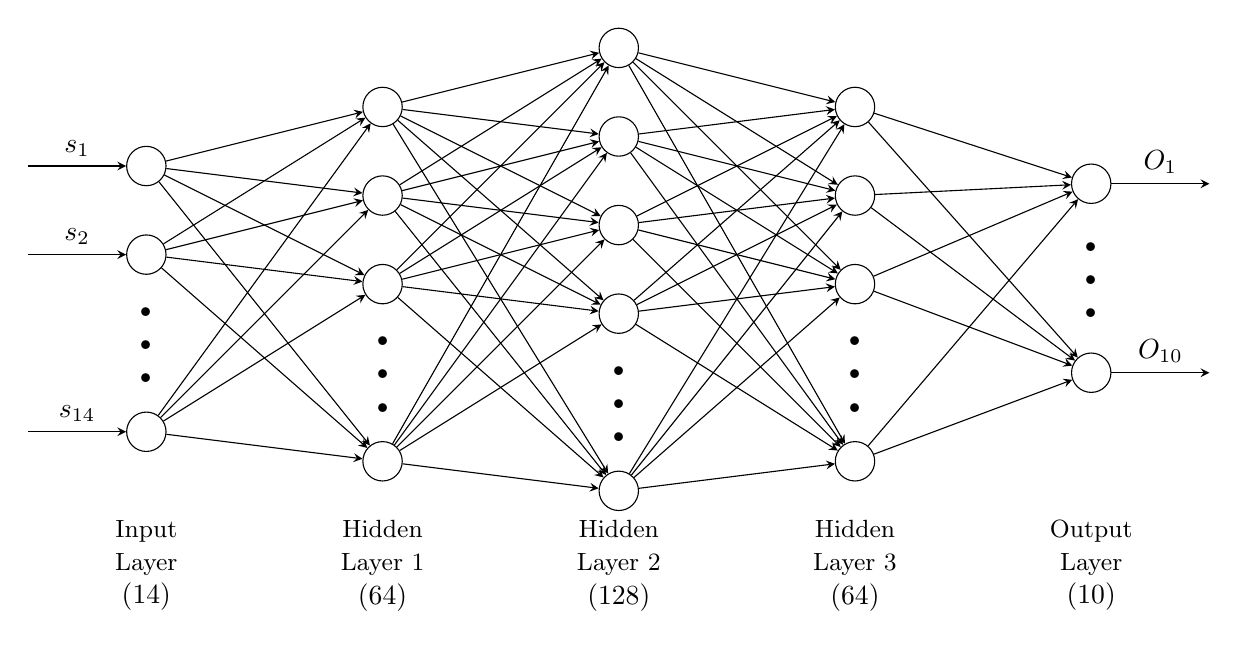
\begin{tikzpicture}[x=1.5cm, y=1.5cm, >=stealth, auto]
    
        \foreach \m/\l [count=\y] in {1,2,missing,3}
          \node [every neuron/.try, neuron \m/.try] (input-\m) at (0,2-\y*.75) {};
        \foreach \m [count=\y] in {1,2,3,missing,4}
          \node [every neuron/.try, neuron \m/.try ] (hidden1-\m) at (2,2.5-\y*0.75) {};
        \foreach \m [count=\y] in {1,2,3,4,missing,5}
          \node [every neuron/.try, neuron \m/.try ] (hidden2-\m) at (4,3-\y*0.75) {};
        \foreach \m [count=\y] in {1,2,3,missing,4}
          \node [every neuron/.try, neuron \m/.try ] (hidden3-\m) at (6,2.5-\y*.75) {};
        \foreach \m [count=\y] in {1,missing,2}
          \node [every neuron/.try, neuron \m/.try ] (output-\m) at (8,1.9-\y*.8) {};
        \foreach \l [count=\i] in {1,2,14}
          \draw [<-] (input-\i) -- ++(-1,0)
            node [above, midway] {$s_{\l}$};
        \foreach \l [count=\i] in {1,10}
          \draw [->] (output-\i) -- ++(1,0)
            node [above, midway] {$O_{\l}$};
        \foreach \i in {1,...,3}
          \foreach \j in {1,...,4}
            \draw [->] (input-\i) -- (hidden1-\j);
        \foreach \i in {1,...,4}
          \foreach \j in {1,...,5}
            \draw [->] (hidden1-\i) -- (hidden2-\j);
        \foreach \i in {1,...,5}
          \foreach \j in {1,...,4}
            \draw [->] (hidden2-\i) -- (hidden3-\j);
        \foreach \i in {1,...,4}
          \foreach \j in {1,...,2}
            \draw [->] (hidden3-\i) -- (output-\j);
        \foreach \l [count=\x from 0] in {\small Input \\\small Layer\\(14) ,\small Hidden \\\small Layer 1\\(64), \small Hidden \\\small Layer 2\\(128), \small Hidden \\\small Layer 3\\(64), \small Output \\\small Layer\\(10)}
          \node [align=center, below, yshift=-5.5cm] at (\x*2,2) {\l};
    \end{tikzpicture}
    \caption{Neural network structure of surrogate model}
    \label{fig:NN}
\end{figure}
        % \foreach \l [count=\i] in {1,2,3,64}
        %   \node [above] at (hidden1-\i.north) {$H_{1,\l}$};
        % \foreach \l [count=\i] in {1,2,3,4,128}
        %   \node [above] at (hidden2-\i.north) {$H_{2,\l}$};
        % \foreach \l [count=\i] in {1,2,3,64}
        %   \node [above] at (hidden3-\i.north) {$H_{3,\l}$};

DNNs are particularly adept at capturing intricate and complex relationships within data, making them well-suited for a wide range of applications, including image recognition, natural language processing, and more. In contrast, \ac{RNN}, characterized by loops in their structure, are ideal for handling sequential and temporal data, incorporating information from previous time steps to model temporal dynamics. Each neuron within an RNN not only processes the current input but also incorporates information from previous time steps. This inherent recurrence equips RNNs to capture and model temporal dynamics, which is essential for scenarios where actions influence subsequent states over time. RNNs employ loops to create a feedback mechanism where the output from one step becomes the input for the next. This cyclic connectivity enables RNNs to maintain a form of memory across different time steps. As an evolution of the RNN architecture, \ac{LSTM} layers incorporate specialized memory cells and gating mechanisms that enable them to selectively retain or forget information over extended sequences. These mechanisms regulate the flow of information through the network, allowing it to selectively remember or forget information over longer sequences.
\tikzset{%
  every neuron/.style={
    circle,
    draw,
    minimum size=0.5cm
  },
  neuron missing/.style={
    draw=none, 
    scale=3,
    text height=0.333cm,
    execute at begin node=\color{black}$\vdots$
  },
  rect neuron/.style={ % Define the style for rectangle nodes
  rectangle,
  draw,
  minimum size=0.5cm,
  align=center, 
  },
  cross/.style={
    path picture={
      \draw[black]
        (path picture bounding box.south east) -- (path picture bounding box.north west)
        (path picture bounding box.south west) -- (path picture bounding box.north east);
    }
  },
}

\begin{figure}[ht]
\centering
    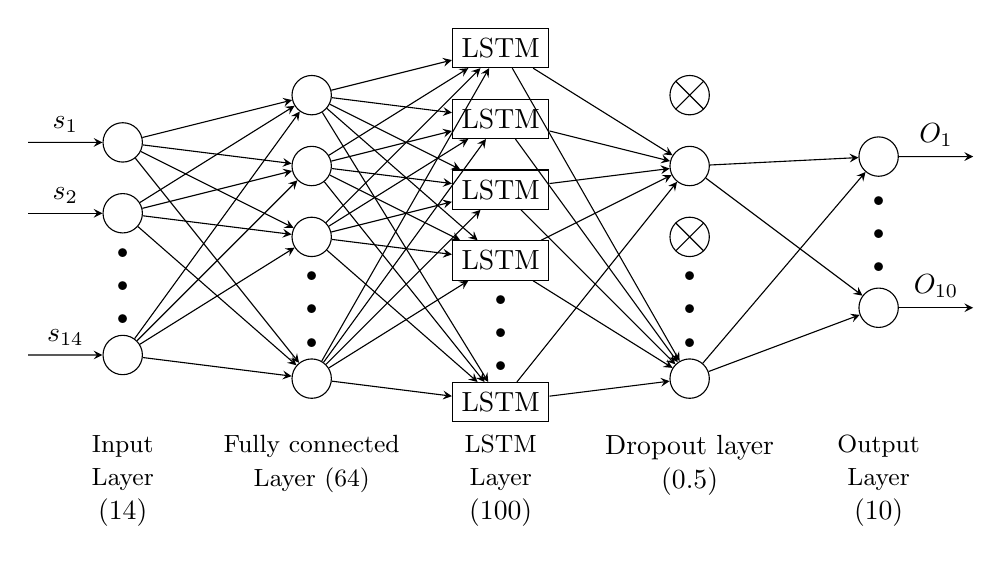
\begin{tikzpicture}[x=1.5cm, y=1.5cm, >=stealth, auto, scale=0.8]
        \foreach \m/\l [count=\y] in {1,2,missing,3}
          \node [every neuron/.try, neuron \m/.try] (input-\m) at (0,2-\y*.75) {};
        \foreach \m [count=\y] in {1,2,3,missing,4}
          \node [every neuron/.try, neuron \m/.try ] (hidden1-\m) at (2,2.5-\y*0.75) {};
        \node [rect neuron/.try, neuron 1/.try] (hidden2-1) at (4,3-1*0.75) {LSTM};
        \node [rect neuron/.try, neuron 2/.try] (hidden2-2) at (4,3-2*0.75) {LSTM};
        \node [rect neuron/.try, neuron 3/.try] (hidden2-3) at (4,3-3*0.75) {LSTM};
        \node [rect neuron/.try, neuron 4/.try] (hidden2-4) at (4,3-4*0.75) {LSTM};
        \node [rect neuron/.try, neuron missing/.try] (hidden2-missing) at (4,3-5*0.75) {};
        \node [rect neuron/.try, neuron 5/.try] (hidden2-5) at (4,3-6*0.75) {LSTM};

        % Dropout Layer
        \node [every neuron/.try, neuron 1/.try ] (dropout-1) at (6,2.5-2*0.75) {};
        \node [every neuron/.try, neuron missing/.try ] (dropout-missing) at (6,2.5-4*0.75) {};
        \node [every neuron/.try, neuron 1/.try ] (dropout-2) at (6,2.5-5*0.75) {};
        \node [every neuron/.try, neuron 1/.try, cross] (dropouted-1) at (6,2.5-1*0.75) {};
        \node [every neuron/.try, neuron 1/.try, cross] (dropouted-2) at (6,2.5-3*0.75) {};
        \foreach \m [count=\y] in {1,missing,2}
          \node [every neuron/.try, neuron \m/.try] (output-\m) at (8,1.9-\y*.8) {};
        \foreach \l [count=\i] in {1,2,14}
          \draw [<-] (input-\i) -- ++(-1,0)
            node [above, midway] {$s_{\l}$};
        \foreach \l [count=\i] in {1,10}
          \draw [->] (output-\i) -- ++(1,0)
            node [above, midway] {$O_{\l}$};
    
        \foreach \i in {1,...,3}
          \foreach \j in {1,...,4}
            \draw [->] (input-\i) -- (hidden1-\j);
        \foreach \i in {1,...,4}
          \foreach \j in {1,...,5}
            \draw [->] (hidden1-\i) -- (hidden2-\j);
        \foreach \i in {1,...,5}
          \foreach \j in {1,...,2}
            \draw [->] (hidden2-\i) -- (dropout-\j);
        \foreach \i in {1,...,2}
          \foreach \j in {1,...,2}
            \draw [->] (dropout-\i) -- (output-\j);
        \foreach \l [count=\x from 0] in {\small Input \\\small Layer\\(14), \small Fully connected \\\small Layer (64), \small LSTM \\\small Layer \\(100), Dropout layer \\(0.5), \small Output \\\small Layer\\(10)}
          \node [align=center, below, yshift=-4.5cm] at (\x*2,2) {\l};
    \end{tikzpicture}
    \caption{\ac{LSTM} \ac{RNN} Architecture. The figure illustrates the architecture of an LSTM-based  RNN. The initial layer comprises the input data, followed by a fully connected layer featuring 64 neurons. Subsequently, the fully connected layer is seamlessly activated by a \ac{ReLU} function before connected to a bidirectional LSTM layer with 100 hidden units. A Dropout layer with 0.5 probability is strategically incorporated before the output layers. }
    \label{fig:lstmstruct}
\end{figure}
        % \foreach \l [count=\i] in {1,2,3,64}
        %   \node [above] at (hidden1-\i.north) {$H_{1,\l}$};
        % \foreach \l [count=\i] in {1,2,3,4,128}
        %   \node [above] at (hidden2-\i.north) {$H_{2,\l}$};
        % \foreach \l [count=\i] in {1,2,3,64}
        %   \node [above] at (hidden3-\i.north) {$H_{3,\l}$};

In the context of the SoftQ surrogate model, a bidirectional LSTM architecture is also adopted, involving two distinct LSTM layers. The first layer processes the sequence in the traditional forward direction, while the second layer processes it in reverse. This bidirectional approach enhances the model's ability to capture bidirectional dependencies within the data. The architecture of the bidirectional LSTM RNN is visually depicted in Fig. \ref{fig:lstmstruct}. In addition to the LSTM layer, a dropout layer with a dropout rate of 50\% is incorporated into the architecture to enhance robustness and generalization capabilities. The dropout layer is a regularization technique that helps prevent overfitting by randomly setting a portion of the input neurons to zero during training.

With the architectural groundwork laid, 15\% of the training data was reserved for validation purposes, and the loss and \ac{RMSE} of the training is shown in Fig. \ref{fig:train2net}(a) and (c). Following this validation stage, the network was evaluated with some manual trot gait test data, the evaluation results are shown in Fig. \ref{fig:comp2net}.

\subsection{Optimization Algorithms}
Furthermore, it is essential to emphasize that alongside architectural considerations, the choice of optimization algorithms holds significant importance before the commencement of the training process. These algorithms steer the iterative parameter updates that guide the model towards convergence. Popular optimization algorithms include \ac{SGDM}, \ac{Adam}, and \ac{RMSProp}. These algorithms adjust the weights of the model based on the gradients of the loss function with respect to the parameters. They help to guide the model towards finding optimal parameter values that minimize the loss function.

\ac{SGDM} augments the standard Stochastic Gradient Descent (SGD) by introducing a momentum term. This term incorporates the weighted average of the previous gradients to determine the direction of the parameter updates. This addition imparts momentum to the optimization process, allowing for smoother convergence by reducing the oscillations that can occur during gradient updates. The momentum term helps to accelerate the movement along shallow directions while dampening oscillations in steep directions. 

\ac{Adam} is an optimization algorithm that combines the advantages of both momentum-based methods and adaptive learning rates. It maintains exponentially decaying moving averages of both past gradients and past squared gradients. These moving averages are used to compute adaptive learning rates for individual parameters. Additionally, \ac{Adam} employs bias correction mechanisms to counteract potential bias towards zero at the beginning of training. By adjusting the learning rates dynamically based on the historical gradients, \ac{Adam} enhances convergence speed and adaptability across varying gradients.

\ac{RMSProp} is an optimization technique designed to address the challenges of learning rate selection in \ac{SGDM}. It maintains an exponentially decaying average of squared gradients for each parameter. The learning rate is then divided by the square root of this average, which normalizes the learning rate by the historical gradient magnitudes. This adaptive learning rate adjustment helps to mitigate the problem of diminishing or exploding gradients.

\begin{figure}[htb]
    \centering
    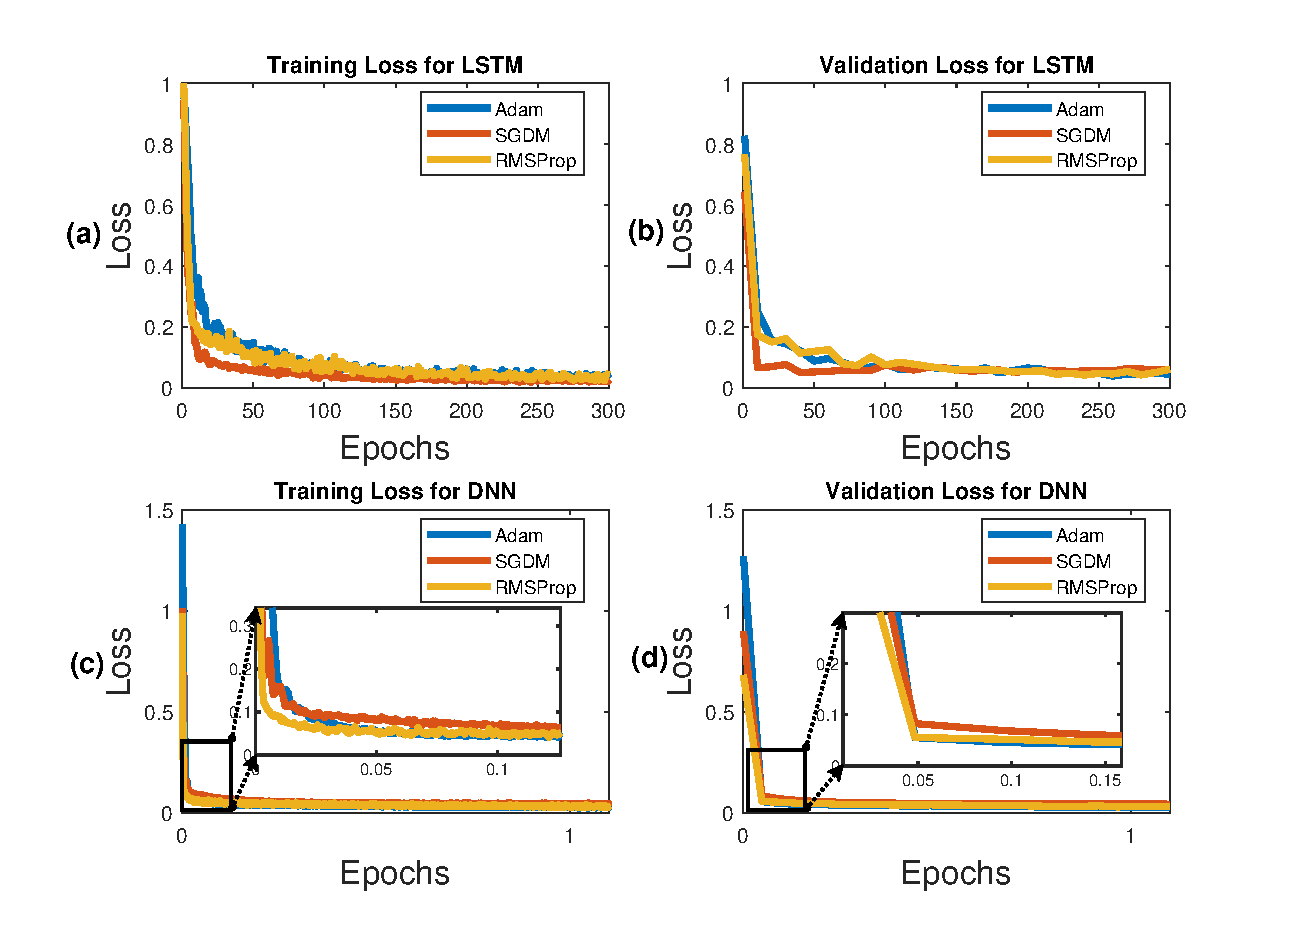
\includegraphics[width=\linewidth]{img/chap4/comp_op.eps}
    \caption{Comparison of Training Trajectories with Different Optimization Algorithms. The figure illustrates the training trajectories of two applied architectures while employing three different optimization algorithms: \ac{SGDM}, \ac{Adam}, \ac{RMSProp}. (a) Training loss and (b) validation loss for the bidirectional \ac{LSTM}-based \ac{RNN} architecture, (c) training loss (d) validation loss for the \ac{DNN} architecture.}
    \label{fig:comp3op}
\end{figure}

By implementing all three optimization algorithms in two networks, a comprehensive exploration was undertaken to discern the most suitable optimization strategy for the training of the surrogate model. This comprehensive approach facilitated a comprehensive assessment of each algorithm's impact on the training process and subsequent model performance. Specifically, the training was performed on both the bidirectional LSTM-RNN and DNN architectures, maintaining a consistent learning rate of 0.001. The training data was shuffled at the end of each epoch, and a mini-batch size of 512 was utilized. The training trajectories of the bidirectional LSTM-RNN and DNN networks, encompassing the utilization of the three optimization algorithms, are visually depicted in Figure \ref{fig:comp3op}. 

For the bidirectional LSTM-based RNN architecture, SGDM is the emerged as the optimal choice due to its remarkable ability to achieve the lowest training loss and converge rapidly. It exhibited both the fastest convergence and the least training loss among the evaluated optimization algorithms. In contrast, for the DNN architecture, Adam optimization took the lead. Adam demonstrated superior performance by learning rapidly and converging to the lowest loss values, both in validation and training. Its ability to efficiently navigate the DNN's training dynamics underscores its suitability for this architecture. Notably, all three optimization algorithms proved to be stable options for training this architecture effectively.

\subsection{Network Validation}
\begin{figure}[htb]
    \centering
    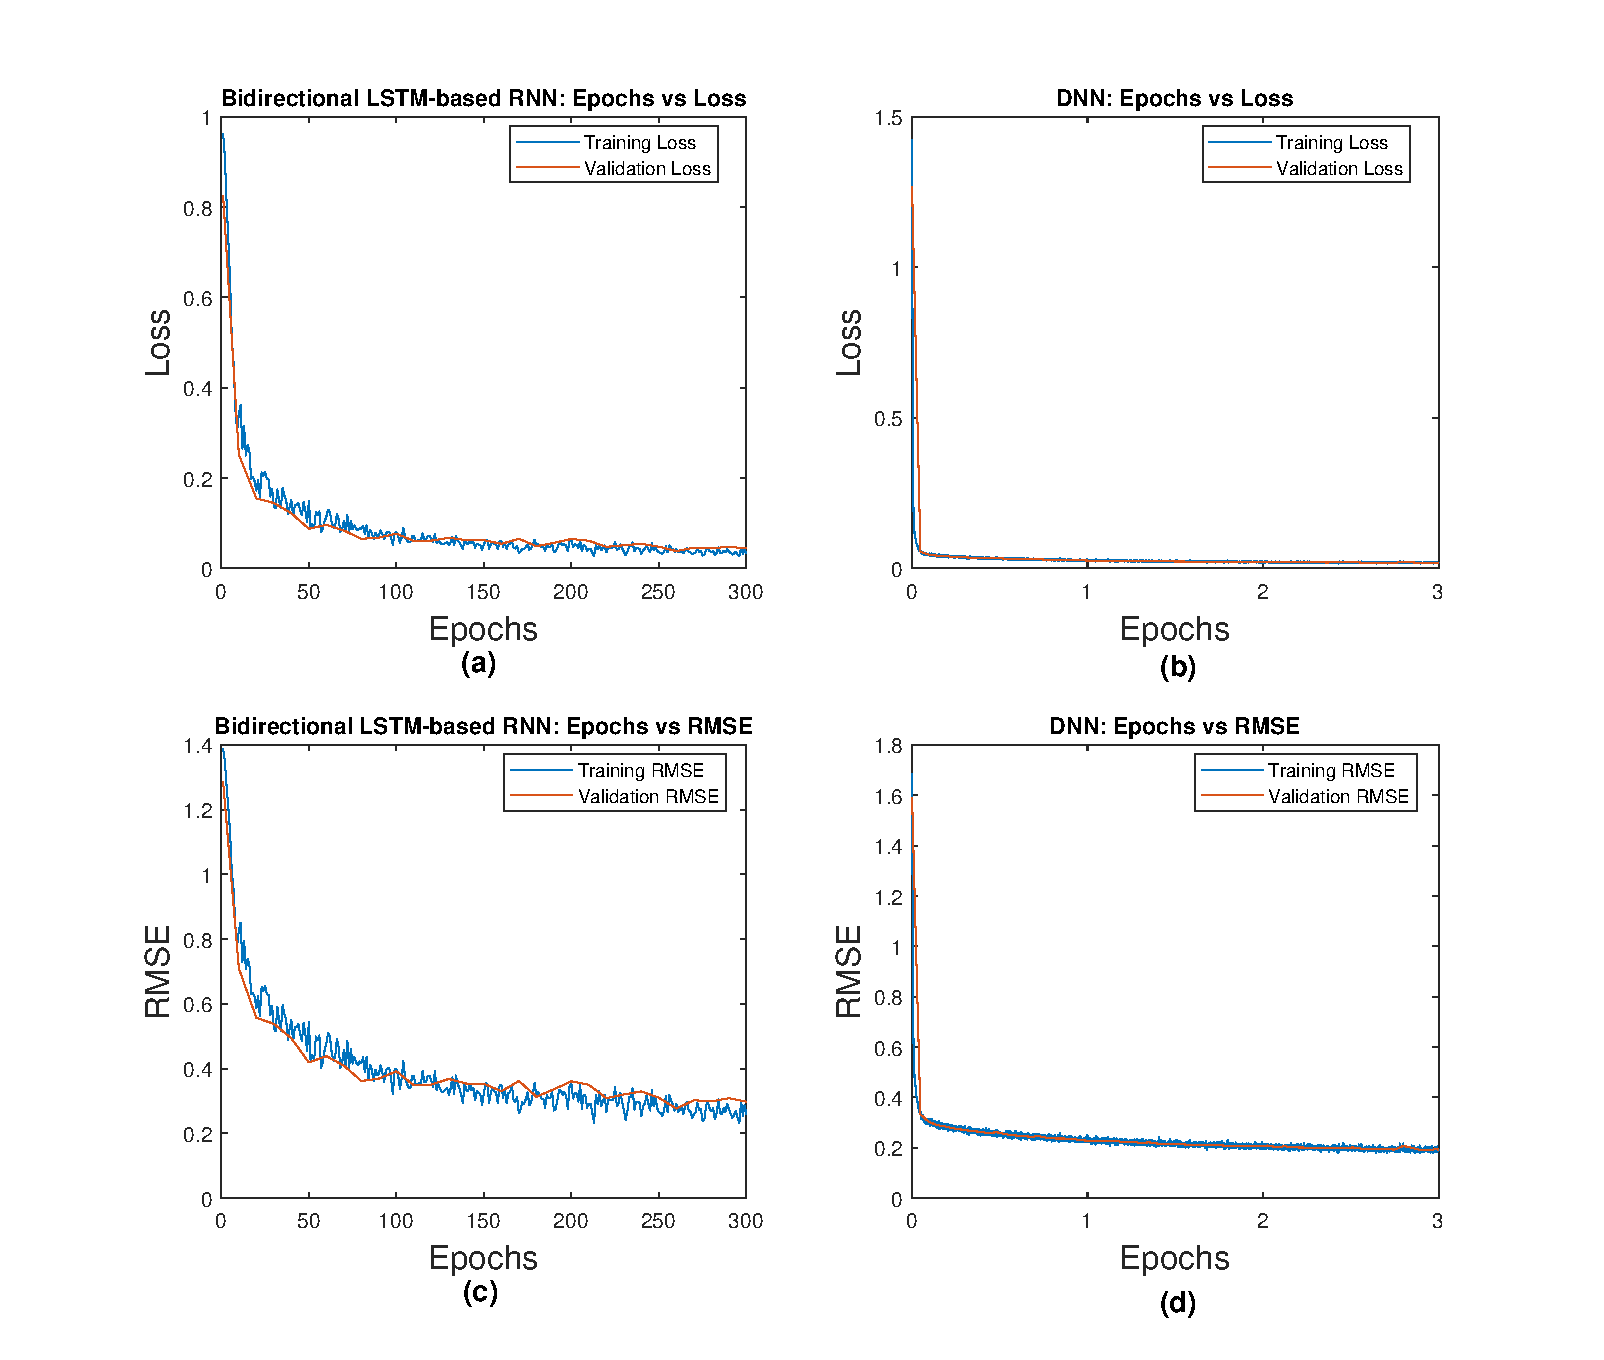
\includegraphics[width=\linewidth]{img/chap4/train_result.eps}
    \caption{Training of bidirectional LSTM-RNN architecture and DNN architecture. (a)-(b) Loss vs epoch for model training with bidirectional LSTM-based and DNN model; (c)-(d) RMSE vs epoch for model training with bidirectional LSTM-based and DNN model.}
    \label{fig:train2net}
\end{figure}

Nonetheless, when comparing the training performance of the bidirectional LSTM-based RNN architecture and the DNN architecture, as illustrated in Figure \ref{fig:train2net}, it becomes evident that the DNN architecture exhibits greater efficiency in terms of data utilization. Notably, the DNN showcases the capability to converge to a lower loss while achieving a reduced \ac{NRMSE}. This underscores the DNN's efficiency in leveraging the provided data and achieving enhanced predictive accuracy with a more compact loss function. Furthermore, evaluated against the real expert trot gait simulation data, the bidirectional LSTM-based RNN architecture achieves an NRMSE of approximately 0.61 for single step prediction, whereas the DNN attains a significantly lower NRMSE of around 0.26. This substantial divergence in NRMSE values highlights the DNN's proficiency in making more accurate predictions on these test cases. A more comprehensive review of the single-step predictions, as compared to the expert trot simulation data, can be observed in Figure \ref{fig:lstm_test} and Figure \ref{fig:DNN_test} in the Appendix. 

\begin{figure}[htb]
    \centering
    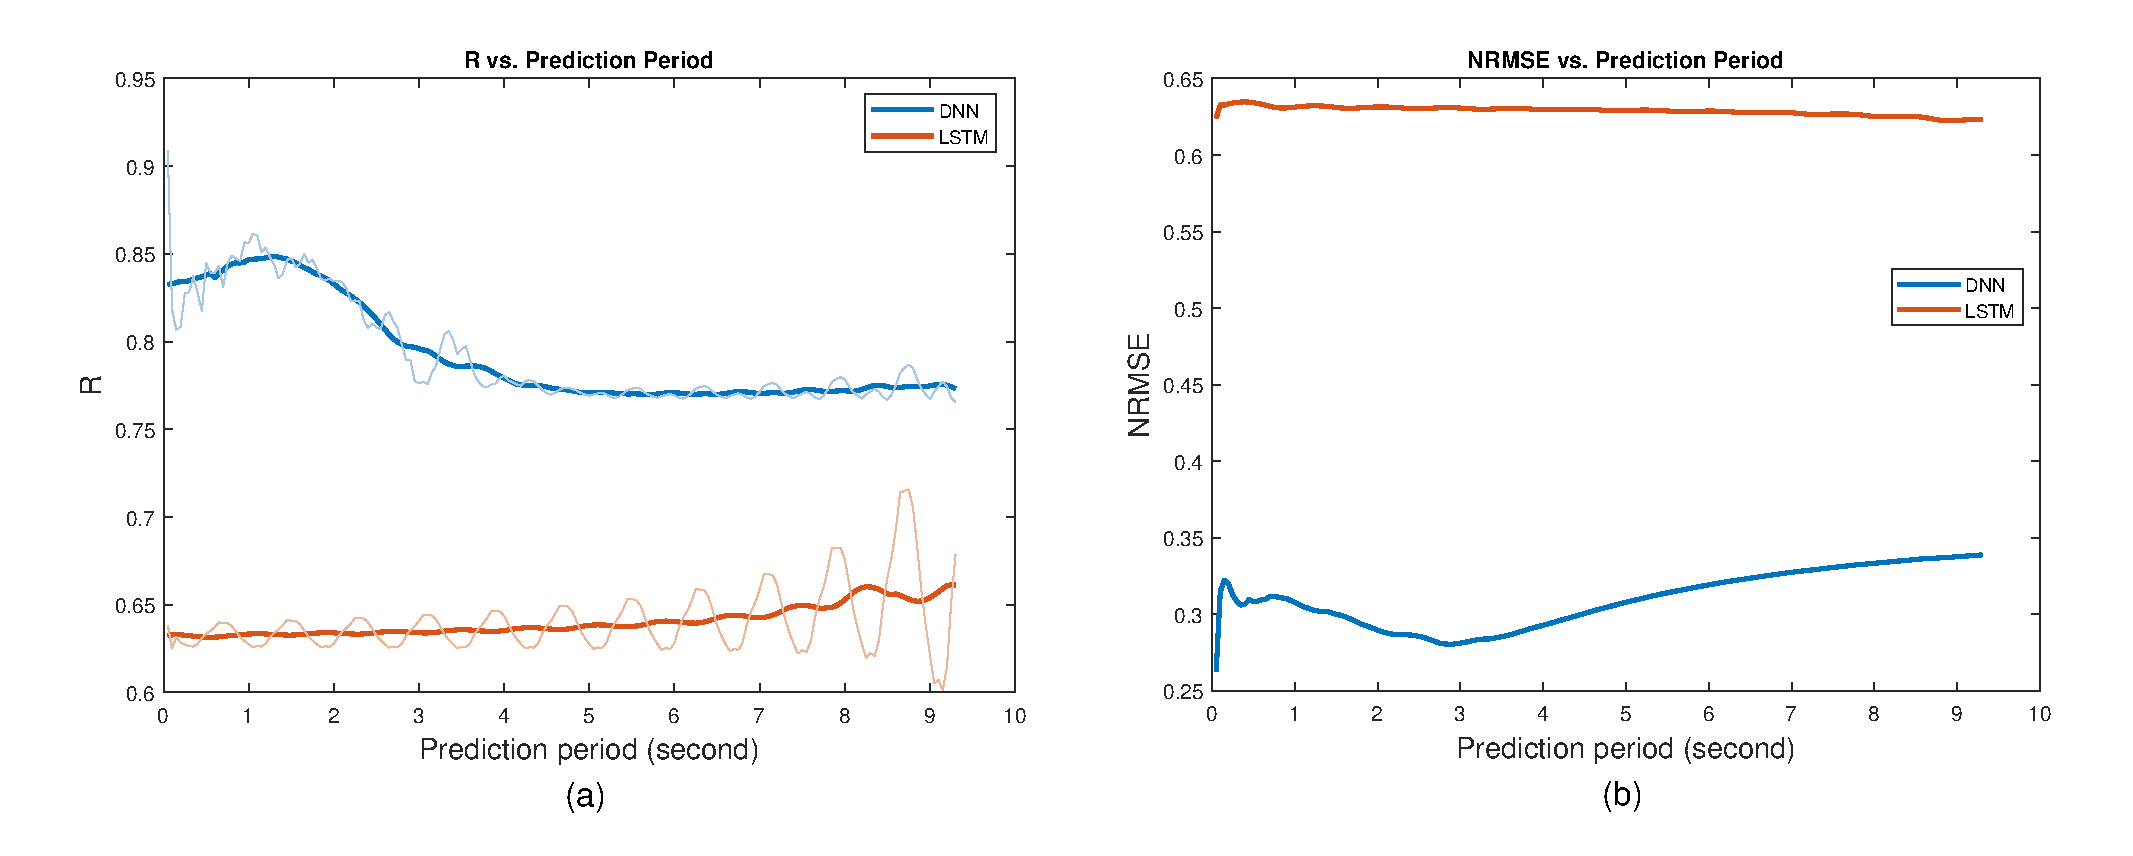
\includegraphics[width=\linewidth]{img/chap4/long2net.eps}
    \caption{Comparison of Long-Term Predictions by Some Expert Gait Data. (a) This figure illustrates the average correlation coefficient ($R$) of long-term predictions between the DNN architecture and the bidirectional LSTM-based RNN architecture. (b) This figure shows the \ac{NRMSE} of long-term predictions between the DNN architecture and the bidirectional LSTM-based RNN architecture.}
    \label{fig:comp2net}
\end{figure}

In addition, an evaluation of the long-term predictions produced by both architectures, as illustrated in Figure \ref{fig:comp2net}, reveals valuable insights. The average correlation coefficient ($R$) for the DNN architecture's single-step predictions exceeded 0.9, maintaining a commendable level of above 0.76 even for predictions spanning 10 seconds. While there was a slight increase in the \ac{NRMSE} for the DNN architecture from 0.26 to 0.35, the \ac{NRMSE} remained relatively stable in the case of the bidirectional LSTM-based RNN. Additionally, it was also observed from the correlation coefficient ($R$) of different prediction steps that the bidirectional LSTM-based RNN architecture did not exhibit substantial drops, demonstrating its stability in predicting long-term and time-series data with consistency. On the other hand, the bidirectional LSTM-based RNN architecture demonstrated a single-step correlation coefficient ($R$) of around 0.64 and an \ac{NRMSE} of approximately 0.62. For long-term predictions, these metrics do not surpass those achieved by the DNN architecture, indicating its limited ability to predict future states with high accuracy. 

LSTM is designed to capture long-term dependencies in sequential data, which can introduce unnecessary complexity when applied to problems with less pronounced sequential patterns. In contrast, DNNs are simpler and may be better suited for situations where data relationships are not strongly sequential. The underlying dynamics of the environment may involve complex and nonlinear relationships. DNNs are well-suited for capturing such intricate patterns, as they can adapt their internal representations to accommodate nonlinearities. While LSTM is a powerful choice for tasks with strong sequential dependencies, it may not be the best fit for problems where data relationships are less sequential. In this particular case, the characteristics of the problem favored the DNN architecture. LSTM, while proficient in handling sequential dependencies, may not excel in capturing these nonlinear relationships. While LSTM is well-regarded for handling sequential data, it may not always be the optimal choice. The DNN's efficiency, simplicity, ability to capture nonlinear patterns, and stability in long-term predictions made it the preferred architecture for this particular task of surrogate model training. Therefore, the DNN architecture optimized with the Adam optimization algorithm emerges as a promising choice for surrogate model training.

\subsection{Dataset Size}
The neural network's architecture, as discussed earlier, provides the framework for representing the complex relationships within the soft quadruped robot's behavior. However, the size of dataset remains a critical factor in enabling the neural network to learn effectively and achieve high estimation accuracy. The dataset's size is defined as a sequence of data, where each sequence data refers to the data collected during a sampling session that occurs without any failures. This definition is established to guarantee the consistency and reliability of the data employed in the neural network's training.

A sufficiently large dataset is essential as it provides the neural network with a diverse set of examples that encompass various scenarios and conditions. This diversity allows the network to generalize well and effectively capture the underlying relationships inherent in the dynamics of the soft quadruped robot. The consequence of having a small dataset is the risk of overfitting, where the network memorizes the training examples but does not truly comprehend the underlying patterns. Conversely, a larger dataset should aid the network in learning these underlying patterns more comprehensively and reduce the risk of overfitting. 

In Figure \ref{fig:datasize}, the average results of 5 long-prediction tests with different dataset size are shown. The correlation coefficient ($R$) remains similar at the single-step prediction level, but for long-term prediction, R increases significantly as the dataset size grows from 20 to around 220 sequences of data. It is worth noting that our analysis identifies oscillations in the correlation coefficient ($R$). These oscillations can be attributed to the presence of an oscillation gait pattern within the data. This gait pattern introduces fluctuations in the predictions at different time steps. Furthermore, we observe that such oscillations are more pronounced when using LSTM networks. This behavior can be attributed to the LSTM's focus on capturing long-term dynamics, potentially overlooking instantaneous dynamics.

In addition to the correlation coefficient, the prediction accuracy was also assessed using \ac{NRMSE}. The findings reveal a consistent trend: the NRMSE decreases as the dataset size grows from 20 sequences to around 280 sequences. These observations indicate that a larger dataset contributes to improved generalization, enhancing the network's ability to accurately estimate the behavior of the soft quadruped robot across a broader range of situations, including those has not encountered during sampling. This becomes particularly crucial when deploying the surrogate model in real-world scenarios where conditions may vary.

However, it's noteworthy that the trend reverses after 300 sequences of data and worsens further with 3000 sequences of data. The reason for the decline in performance with more data could be attributed to the fact that the random action data collected may not adequately characterize the useful information about the robot's dynamics. This could be due to the imbalanced distribution of data, with fewer samples representing high walking velocity, leading to the diminishing returns of adding more data in this form.
\begin{figure}[htb]
    \centering
    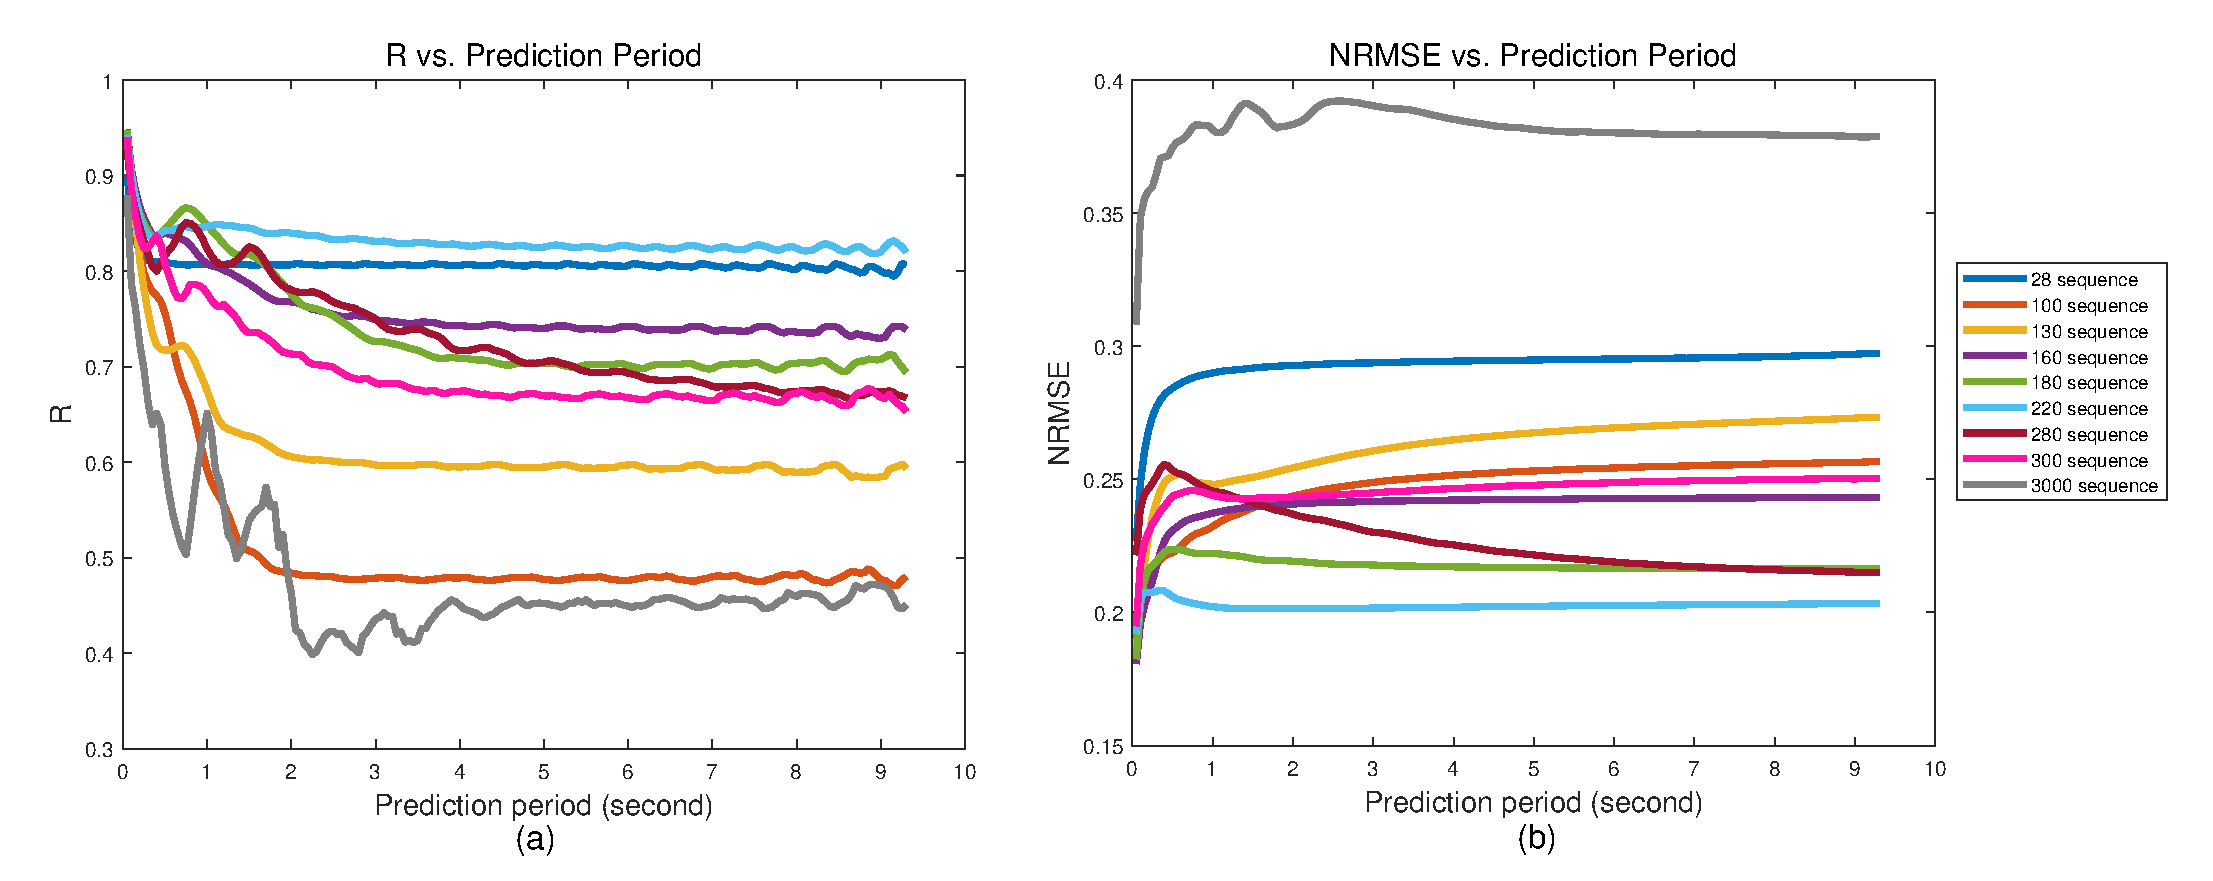
\includegraphics[width=\linewidth]{img/chap4/datasize.eps}
    \caption{Comparison of Different Data Size of Dataset $\mathcal{D}$ in Long-Term Predictions using some expert trot gait data. (a) This figure illustrates the average correlation coefficient ($R$) of long-term predictions between the DNN architecture and the bidirectional LSTM-based RNN architecture. (b) This figure shows the \ac{NRMSE} of long-term predictions between the DNN architecture and the bidirectional LSTM-based RNN architecture.}
    \label{fig:datasize}
\end{figure}

It's crucial to strike a balance between dataset size and the associated computational resources and time required for training. Collecting and curating a substantial dataset demands significant effort and resources, and training a neural network on a large dataset can be computationally intensive. Therefore, careful consideration is required to determine an appropriate dataset size that aligns with the available resources while still achieving the desired level of accuracy and generalization. Based on these observations, selecting a dataset size approximately 20 times the dimensions of the observation data seems to strike a reasonable balance for the surrogate model in this thesis, which means about 200 sequences of data in this thesis.

\section{Model-based RL Algorithm}
After successfully training the surrogate model, the next phase of this thesis involves the application of \ac{MBRL} algorithms to further advance the research objectives. As previously discussed in Chapter \ref{chap2}, the \ac{SAC} algorithm has been selected due to its advantages in promoting efficient exploration and its compatibility with continuous action spaces. 

SAC addresses the challenge of dealing with continuous action spaces by incorporating an actor network that explicitly represents the policy function. This actor network is parameterized to output a probability distribution over actions, typically modeled as a Gaussian distribution with mean and standard deviation. SAC learns both the Q-function and the policy (actor) simultaneously through a combination of entropy-regularized policy optimization and Q-value estimation.

\subsection{SAC Algorithm}
The \ac{SAC} algorithm builds upon the principles of Actor-Critic but introduces a significant enhancement. To find an optimal gait controller through RL, the surrogate model is employed as an environment model within the framework of a Markov Decision Process ($\mathcal{S}, \mathcal{A}, P, r$). In this construct:
\begin{itemize} 
    \item $\mathcal{S}$ and $\mathcal{A}$ characterize the continous state and action spaces, respectively.
    \item The transition function $P(\mathbf{s}_{t+1} | \mathbf{s}_t, \mathbf{a}_t): \mathcal{S} \times \mathcal{A} \times \mathcal{S} \rightarrow [0,+\infty)$ encapsulates the probability density governing an agent's transition from the current state $s_t \in S$ to a subsequent state $\mathbf{s}_{t+1} \in \mathcal{S}$ upon executing action $\mathbf{a}_t \in \mathcal{A}$. This function encapsulates the dynamics of the environment.
    \item Following the execution of action $\mathbf{a}_t$ within state $\mathbf{s}_t$, the agent is rewarded with an immediate feedback $r_t := r(\mathbf{s}_t, \mathbf{a}_t)$. The reward function $r: \mathcal{S} \times \mathcal{S} \to \mathbb{R}$ quantifies the desirability of an action within a given state.
\end{itemize}

The central objective of SAC is to derive a policy that maximizes the cumulative expected reward while also taking into account the entropy of the policy distribution. Specifically, if $X$ is a random variable and its probability density function is $p$, then its entropy $H(X)$ is defined as $H(X) = \mathbb{E}_{x\sim p}[-\ln p(x)]$, then the degree of stochasticity of a policy $\pi$ in a state $\mathbf{s}_t$ could be represented as $H(\pi(\cdot|\mathbf{s}_t)) = \mathbb{E}_\pi[-\ln \pi(\mathbf{a}_t|\mathbf{s}_t)]$. Policy entropy measures the randomness of the actions available to the agent, with higher entropy values indicating greater uncertainty. By including the entropy value in the objective function, exploration during training is encouraged, mitigating the risk of converging to a locally optimal policy. A non-deterministic control policy $\pi$ provides the conditional probability density $\pi(\mathbf{a}_t|\mathbf{s}_t)$ of taking action $\mathbf{a}_t$ in a known state $\mathbf{s}_t$. The goal is to find a stochastic policy that maximizes the sum of rewards and entropy. 

According to this Soft Bellman equation\cite{haarnojaSoftActorCriticOffPolicy2018}, the process of Soft Policy Iteration can ultimately converge to the Soft $Q$ function associated with policy $\pi$. Then in the policy improvement step, the policy is updated towards the exponential of the new soft $Q$ function. The iterative process of alternating between Soft policy evaluation and Soft policy improvement allows the final policy to converge to the optimal policy, as dictated by the objectives of maximum entropy reinforcement learning. In cases involving continuous spaces, it becomes necessary to approximate these iterations by parameterizing the $Q$ function and the policy $\pi$. In the maximum entropy RL, the problem can be defined to find the optimal policy $\pi^*$ each visited state, with the form of 
\begin{equation}
    \pi^* = \arg\max_\pi\mathbb{E}_\pi [\sum_t r(\mathbf{s}_t,\mathbf{a}_t)+\alpha H(\pi(\cdot|\mathbf{s}_t))]
    \label{eq:bellman}
\end{equation} 
where $\alpha$ is the entropy regularization coefficient that explicitly controls the trade-off between exploration and exploitation. It determines the relative importance between the entropy term against the reward, and a higher $\alpha$ corresponds to higher exploration. 

In Soft Policy Iteration, the Soft Bellman equation plays a pivotal role in evaluating and improving the control policy. This equation calculates the expected reward for taking an action $\mathbf{a}_t$ in a state $\mathbf{s}_t$ and then following the policy $\pi$ with a discount factor $\gamma$.  This $Q$ function, which assesses the quality of a control policy, can be expressed as:
\begin{equation}
    Q_\pi(\mathbf{s}_t,\mathbf{a}_t) = r(\mathbf{s}_t,\mathbf{a}_t) + \gamma\mathbb{E}_{\pi}[V(\mathbf{s}_{t+1})]
    \label{eq:Q}
\end{equation} 
Next, the value function $V_\pi(\mathbf{s}_t)$ is defined to represent the expected cumulative reward when following policy $\pi$ from state $\mathbf{s}_t$. It takes into account the Soft $Q$ function and incorporates an entropy term with a temerature parameter $\alpha$:
\begin{equation}
    V_\pi(\mathbf{s}_t) = \mathbb{E}_{\mathbf{a}_t\sim \pi}[Q_\pi(\mathbf{s}_t,\mathbf{a}_t)] + H(\pi(\cdot|\mathbf{s}_t)) = \mathbb{E}_{\mathbf{a}_t\sim \pi}[Q_\pi(\mathbf{s}_t,\mathbf{a}_t) - \alpha\ln\pi(\mathbf{a}_t|\mathbf{s}_t)]
    \label{eq:valuef}
\end{equation}

For environments in continuous state and action spaces, the SAC algorithm employs Gaussian mixtures with mean and variance through the neural networks to model both the soft Q-function critic and the policy actor. Specifically, two action-value $Q$ functions are modeled, each parameterized by $\omega_1$ and $\omega_2$ and a policy function $\pi$, parameterized by $\phi$. SAC follows the concept of Double Deep Q-Network (DQN), using two networks and selecting the one with the smaller value to mitigate value overestimation issues. Both networks provide independent estimations of the value function through $Q_1(\mathbf{s}_t, \mathbf{a}_t)$ and $Q_2(\mathbf{s}_t, \mathbf{a}_t)$. Additionally, corresponding target networks, $Q_{\omega_1}(\mathbf{s}_t, \mathbf{a}_t)$ and $Q_{\omega_2}(\mathbf{s}_t, \mathbf{a}_t)$, are created to enhance optimization stability. During the update of both the $Q$ value function and the policy function, the minimum of the two target $Q$ functions is used for temporal difference target calculation. The loss function for the $Q$ functions, denoted as $L_Q(\omega)$, aims to minimize the soft Bellman residual: 
\begin{equation}
    \begin{aligned}
    &L_Q(\omega) = \mathbb{E}_{(\mathbf{s}_t, \mathbf{a}_t, r_t, \mathbf{s}_{t+1}) \sim R}\bigg[\frac{1}{2}\bigg(Q_\omega(\mathbf{s}_t,\mathbf{a}_t)-(r_t+\gamma V_\omega^- (\mathbf{s}_{t+1}))\bigg)^2\bigg]\\
    &=\mathbb{E}_{(\mathbf{s}_t, \mathbf{a}_t, r_t, \mathbf{s}_{t+1}) \sim R,\;\mathbf{a}_{t+1} \sim \pi_\phi(\cdot|\mathbf{s}_{t+1})}\bigg[\frac{1}{2}\bigg(Q_\omega(\mathbf{s}_t,\mathbf{a}_t)-(r_t+\gamma(\min_{j=1,2}Q_{\omega_j}(\mathbf{s}_t,\mathbf{a}_t)-\alpha\ln\pi(\mathbf{a}_{t+1}|\mathbf{s}_{t+1}))\bigg)^2\bigg]
    \end{aligned}
    \label{eq:lossSAC}
\end{equation}
This loss function incorporates the temporal difference error, accounting for the difference between the predicted Q-value and the target value, which is a combination of the immediate reward and the estimated value of the next state. Additionally, the policy entropy term is included in the loss function. The loss function of the policy $\pi$ is obtained from the Kullback-Leibler divergence, which is simplified as: $$L_\pi(\phi)=\mathbb{E}_{\mathbf{s}_t\sim R,\mathbf{a}_t\sim \pi_\phi}[\alpha\ln(\pi_\phi(\mathbf{a}_t|\mathbf{s}_t))-Q_\omega(\mathbf{s}_t,\mathbf{a}_t)]$$The convergence and optimality of this approach have been rigorously established in previous works\cite{haarnojaSoftActorCriticAlgorithms2019, haarnojaSoftActorCriticOffPolicy2018}. 

To adaptively adjust the entropy regularization term, SAC reformulates the RL objective as an optimization problem with constraints. The aim is to maximize the expected return while ensuring that the mean entropy remains above a specified threshold $H_0$: $$\max_\pi\mathbb{E}_\pi \bigg[\sum_t (\mathbf{s}_t, \mathbf{a}_t)\bigg]\:s.t.\:\mathbb{E}_{(\mathbf{s}_t, \mathbf{a}_t)\sim\rho_\pi}[-\ln (\pi_t(\mathbf{a}_t|\mathbf{s}_t))] \geq H_0\;\forall t$$ During the training process, the temperature parameter $\alpha$ is dynamically updated based on the entropy of the current policy, using past experiences. Initially set to 1, $\alpha$ gradually decreases to 0 as the training progresses. That is, maximising the expected return while constraining the mean value of entropy to be greater than $H_0$, the $\alpha$ will be updated by the loss function: $$L_\pi(\alpha) = \mathbb{E}_{\mathbf{s}_t\sim R, \mathbf{a}_t\sim\pi(\cdot|\mathbf{s}_t)} [-\alpha\ln\pi(\mathbf{a}_t|\mathbf{s}_t)-\alpha H_0]$$ This adjustment reduces the emphasis on exploration when evaluating the value function. When the policy's entropy falls below the target value $H_0$, the training objective increases $\alpha$, giving more weight to the policy entropy term and encouraging exploration. Conversely, when the policy's entropy exceeds $H_0$, $\alpha$ decreases, focusing the policy training more on value enhancement.\begin{figure}[htb]
    \centering
    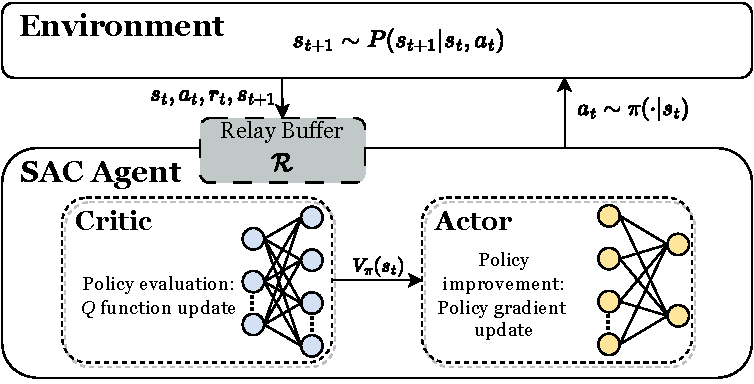
\includegraphics[width=0.9\linewidth]{img/chap4/SAC.pdf}
    \caption{Schematic of the Soft Actor Critic (SAC) method. Reproduced from Ji et al.\cite{jiSynthesizingOptimalGait2022}}
    \label{fig:SAC}
\end{figure}
 

In Figure \ref{fig:SAC}, an overview of this approach to learn a walking gait controller for a quadruped robot using the SAC algorithm is presented. The process begins with initialization, followed by the actor selecting an action $\mathbf{a}_t$ at each training step based on the observation $\mathbf{s}_t$, guided by the policy $\pi(\cdot|\mathbf{s}_t)$. The selected action is executed, allowing the robot to interact with the environment and receive a reward $r_t$ along with the next observation $\mathbf{s}_{t+1}$. These experiences, denoted as ($\mathbf{a}_t, \mathbf{s}_t, r_t, \mathbf{s}_{t+1}$), are stored in the replay buffer $R$ and serve as training data for updating the neural network parameters. The agent periodically updates the parameters in the Q-value network, alternating between the two networks to mitigate value overestimation. Note that the actor–critic connection is represented in the update of the actor policy network, where its update utilizes the minimum of soft state value from target Q networks based on \ref{eq:valuef}. The policy actor network and temperature parameter are also updated through stochastic gradient descent, minimizing the residual across batch samples from the replay buffer $\mathcal{R}$. The update process considers the minimum of soft state values from target Q networks, as described earlier. The learning rate $\lambda$ guides the parameter updates in the descent direction. This iterative process of interaction and learning continues until the gait controller converges to an optimal policy or reaches a predefined maximum number of episodes. To obtain a more comprehensive and in-depth mathematical elucidation, one is advised to consult the primary research articles authored by Haarnoja et al.\cite{haarnojaSoftActorCriticAlgorithms2019, haarnojaSoftActorCriticOffPolicy2018}. This algorithm effectively addresses the challenges of continuous state and action spaces, providing a framework for maximum entropy reinforcement learning in such environments.

\subsection{Agent Specifications and Reward}
In the context of reinforcement learning, the definition of state, action, and reward constitutes a critical phase. This section provides an in-depth exposition of these fundamental aspects.
\subsubsection{State space}
\label{sec:ss}
The first consideration revolves around the definition of the state space, which is defined as the available sensor measurements from the robot. As discussed before, it includes the robot's orientation $\pmb{\theta}(t) =[\theta_x(t),\theta_y(t),\theta_z(t)]\:\in\:\mathbb{R}^3$ with regards to three dimensions, specifically roll, pitch, yaw; the moving velocities $\mathbf{v}(t) =[v_x(t),v_y(t),v_z(t)]\:\in\:\mathbb{R}^3$ along three principal axes, $x$, $y$ and $z$; and the normalized contact force $\mathbf{f}_n(t)=[f_{nFL}(t), f_{nFR}(t), f_{nRR}(t), f_{nRL}(t)]\:\in\:\mathbb{R}^4$ between each foot and ground. The above 10 dimensional measurements provide a comprehensive perspective on the robot's surroundings, enabling us to infer its internal state accurately. Additional insights into the nature and characteristics of these sensor measurements are available in Chapter \ref{chap3}. In addition, due to the computation and communication delays in real-world implementations, these temporal disparities introduce asynchrony between the observation of the environment and the execution of control actions. Notably, this asynchrony challenges the fundamental assumptions underpinning the Markov Decision Process, potentially resulting in substantial performance degradation, particularly in robot locomotion tasks. To address this challenge and ensure the effective modeling of the system's dynamics, a holistic approach is adopted. Specifically, the state representation is augmented by incorporating the action executed during the previous time step, denoted as $\mathbf{a}_{t-1} \in \mathbb{R}^4$. This augmentation empowers the agent to consider the temporal dependencies of its actions and their influence on the current state. Consequently, the state vector, denoted as $\mathbf{s}_t$, assumes an expanded form: $$\mathbf{s}_t =[\pmb{\theta}(t),\mathbf{v}(t),\mathbf{f}_n(t),\mathbf{a}_{t-1}] \:\in\:\mathbb{R}^{14}$$ This enriched state representation equips the agent with an enhanced capacity to model the dynamics of its environment effectively. Furthermore, it enables the agent to grapple with the complexities arising from hardware latency in real-time robotic applications, ultimately advancing the pursuit of optimal gait control.
\subsubsection{Action space}
\label{Sec:as}
As previously elucidated, the locomotion of the robot is intricately governed by an inverse kinematics model, elegantly captured by Equation \ref{eq:value2motor}. In this context, the gait could be meticulously designed to propel the robot forward, with a particular parameterization on diagonal leg pairs. Consequently, the action space is framed around the articulation of these diagonal leg pairs. In precise terms, the action space is defined by two key components, desired bending angles ($\alpha_{b_1}\,,\alpha_{b_2}$) of each diagonal leg pairs and compressed leg length ($z_{l_1}\,,z_{l_2}$) of each diagonal leg pairs, that is $\mathbf{a}_{t} = [\alpha_{b_1}, z_{l_1}, \alpha_{b_2}, z_{l_2}]$. For faster gradient descent, the actor output is normalized between 0 and 1 based on the action spaces derived from the simulation dataset. Thus, the action space is defined as a continuous 4-dimensional space, and a single action $\mathbf{a}_t$ is a vector containing 4 desired motor positions after normalization, i.e., $\mathbf{a}_t \:\in\:[0,1]^4$ Subsequently, the policy network output is transformed using a mapping to reference leg locomotion: $\alpha_{b_{ref}} = 2\alpha_{b_{gain}}(\alpha_b(t) -0.5)$ for bending angle, and $z_{l_{ref}} = z_{l_{gain}}z_l(t)$ for compressed leg length. These transformations allow for the conversion of the actor's output into meaningful references for leg locomotion, thereby enabling the robot to execute the desired gait effectively.
\subsubsection{Reward}
The primary objective in this study is to encourage the robot maintain a straight and stable gait over extended periods. Hence, the objective reward function is formulated and defined as: 
\begin{equation}
    r(\mathbf{s}_t,\mathbf{a}_t) = \epsilon_1\frac{T_s}{T_f} + (1-\epsilon_2|v_x(t)-v_{ref}|)-\epsilon_3\lVert\Ddot{\mathbf{a}_t}\rVert - \epsilon_4\lVert\mathbf{a}_t-\mathbf{\sigma}_{threshold}\rVert - \epsilon_5(\mathbf{a}_t-\frac{\sum_{i=1}^{H}\mathbf{a}_i}{H})^2
    \label{eq:reward}
\end{equation}
In each episode, the control steps continue until the robot falls or the simulation fails. The criteria of failing are identical to that of simulation termination as previously defined in Section \ref{sec3.2}. At each training step, the robot is rewarded with a constant value $\epsilon_1\frac{T_s}{T_f}$ for maintaining balance without triggering any terminal conditions. Here $T_s$ denotes the sampling time of the agent's interaction with the simulation environment, and $T_f$ is the final time of this training in one episode. Instead of applying significant penalties upon episode termination due to undesired states, continuous rewards at each step for the robot's longevity in the task are provided. The accumulated rewards for this term are proportional to the sequence length, effectively motivating the agent to remain upright for extended duration. 

As a walking gait controller, the agent is trained to encourage the robot to consistently move in close alignment with a reference speed $v_{ref}$ along the $x$-axis. To achieve this, a reward component that regulates the forward velocity $v_x(t)$. This component utilizes a shifted absolute value function, with $\epsilon_2$ governing the shape of the reward function. The essential idea  is to stimulate the robot to maintain forward motion with a positive speed while discouraging backward movement (negative speed). Therefore, the choice of $\epsilon_2$ is dependent on the reference speed $v_{ref}$, with a larger magnitude of $\epsilon_2$ favored when $v_{ref}$ decreases. This sharpens the reward decay near $v_{ref}$ and penalizes negative velocities. For simplicity, we set $\epsilon_2 = −1/v_{ref}$ to ensure that the maximum reward is unity, and negative speeds are penalized. 

To promote stable action on motors, a penalty on the large action acceleration $\Ddot{\mathbf{a}_t}$ quantified by $\epsilon_3$ is introduced. This penalty discourages abrupt changes in motor actions, aiming to deliver a stable actuation signal to the motors. The penalty acceleration value is estimated using finite differences of actions from the last three time steps: $$\Ddot{\mathbf{a}_t} = \frac{\mathbf{a}_t+\mathbf{a}_{t-2}-2\mathbf{a}_{t-1}}{T_s^2}$$ Note that $\mathbf{a}_{t-1}$ and $\mathbf{a}_{t-2}$ are not included in the state space at the time step $t$, but is recorded in the robot's memory.

In addition, to ensure stable walking gait control, the excessive bending angles $\alpha_b$ of the robot's leg pairs are penalized, where negative rewards are assigned as $- \epsilon_4\lVert\mathbf{a}_t-\sigma_{threshold}\rVert$, serving as a discouragement for excessive leg bending. $\sigma_{threshold}$ is the threshold for bending angle to prevent simultaneous bending of all four legs. However, it was observed that penalizing leg pairs for excessive bending alone was insufficient. Therefore, an additional penalty term is introduced, which is $ - \epsilon_5(\mathbf{a}_t-\frac{\sum_{i=1}^{H}\mathbf{a}_i}{H})^2$. This term penalizes leg pairs that consistently bend in the same direction over a horizon $H$. In this study, the horizon $H$ is set to 16 time steps based on experimental results. The weighting factor $\pmb{\epsilon} = [\epsilon_1, \epsilon_2, \epsilon_3, \epsilon_4, \epsilon_5]$ objectively defines the emphasis placed on each aspect of the reward function. These values have been thoughtfully selected as $[5, −1/v_{ref}, 0.25, 10, 3]$, aligning with the objective of training the robot effectively.

\subsection{Training Setup}
As previously mentioned, two Q-value critic networks are employed, each complemented by its corresponding target critic network. Their primary purpose is to estimate the $Q$ function as defined in Eq. \ref{eq:Q}. These critic networks share a uniform architecture, characterized by two distinct input components: observations and actions. The observation section undergoes processing through two fully-connected layers, each comprising 128 units. Meanwhile, the action component is managed by a single fully-connected layer with 128 units. The outputs from both sections are concatenated and subsequently channeled through another fully-connected layer featuring 32 units, with the activation function being \ac{ReLU}. The ultimate output of the Q network serves as an estimation of the $Q$ function. 

Concurrently, the actor network utilizes the environment observation as its input. This input is processed through two fully-connected layers, each containing 256 units, and employs ReLU as the activation function. The core responsibility of the actor network is to predict the mean and variance for each action through Gaussian distributions. To ensure that the generated actions fall within the [0, 1] range, the hyperbolic tangent function (tanh) is employed as a squashing function. 

To mitigate the risk of overfitting, the learning rates for both the critic and actor networks are set at 0.002 and 0.001, respectively. The learning rate for the temperature parameter $\alpha$ is kept consistent with the network learning rates, fixed at 0.001. For the sake of stability during updates, the update frequency of the policy network is reduced, with parameters being updated every 3 steps in the simulation. The discount factor $\gamma$ is firmly set at 0.96, as the number of complete steps in a training episode is 50. Furthermore, the target entropy is defined based on the number of actions, with a specific value of $H'=-4$. The batch size is set to 4096 ($2^{12}$), and the size of the replay buffer is 16384 ($2^{14}$). To ensure uniformity in environment initialization, all episodes begin from the same initial state $\mathbf{s}_0$.

\section{Control Architecture Design}
The control architecture design of the soft quadruped robot is a critical component in achieving stable and efficient locomotion. In essence, the control architecture of the soft quadruped robot represents a harmonious synthesis of hardware, software, and sensor integration. This design enables stable and efficient locomotion, with servo motors, the STM32 microcontroller, and seamless communication underpinning precise control. Additionally, sensory observations gathered through a diverse array of sensors empower the robot with heightened environmental perception and adaptability. The Simulink controller, driven by observations and control commands, ensures the robot's actions align with its intended behaviors, ultimately culminating in stable and efficient locomotion. The control architecture of SoftQ is visually depicted in Figure \ref{fig:control}.
\begin{figure}[htb]
    \centering
    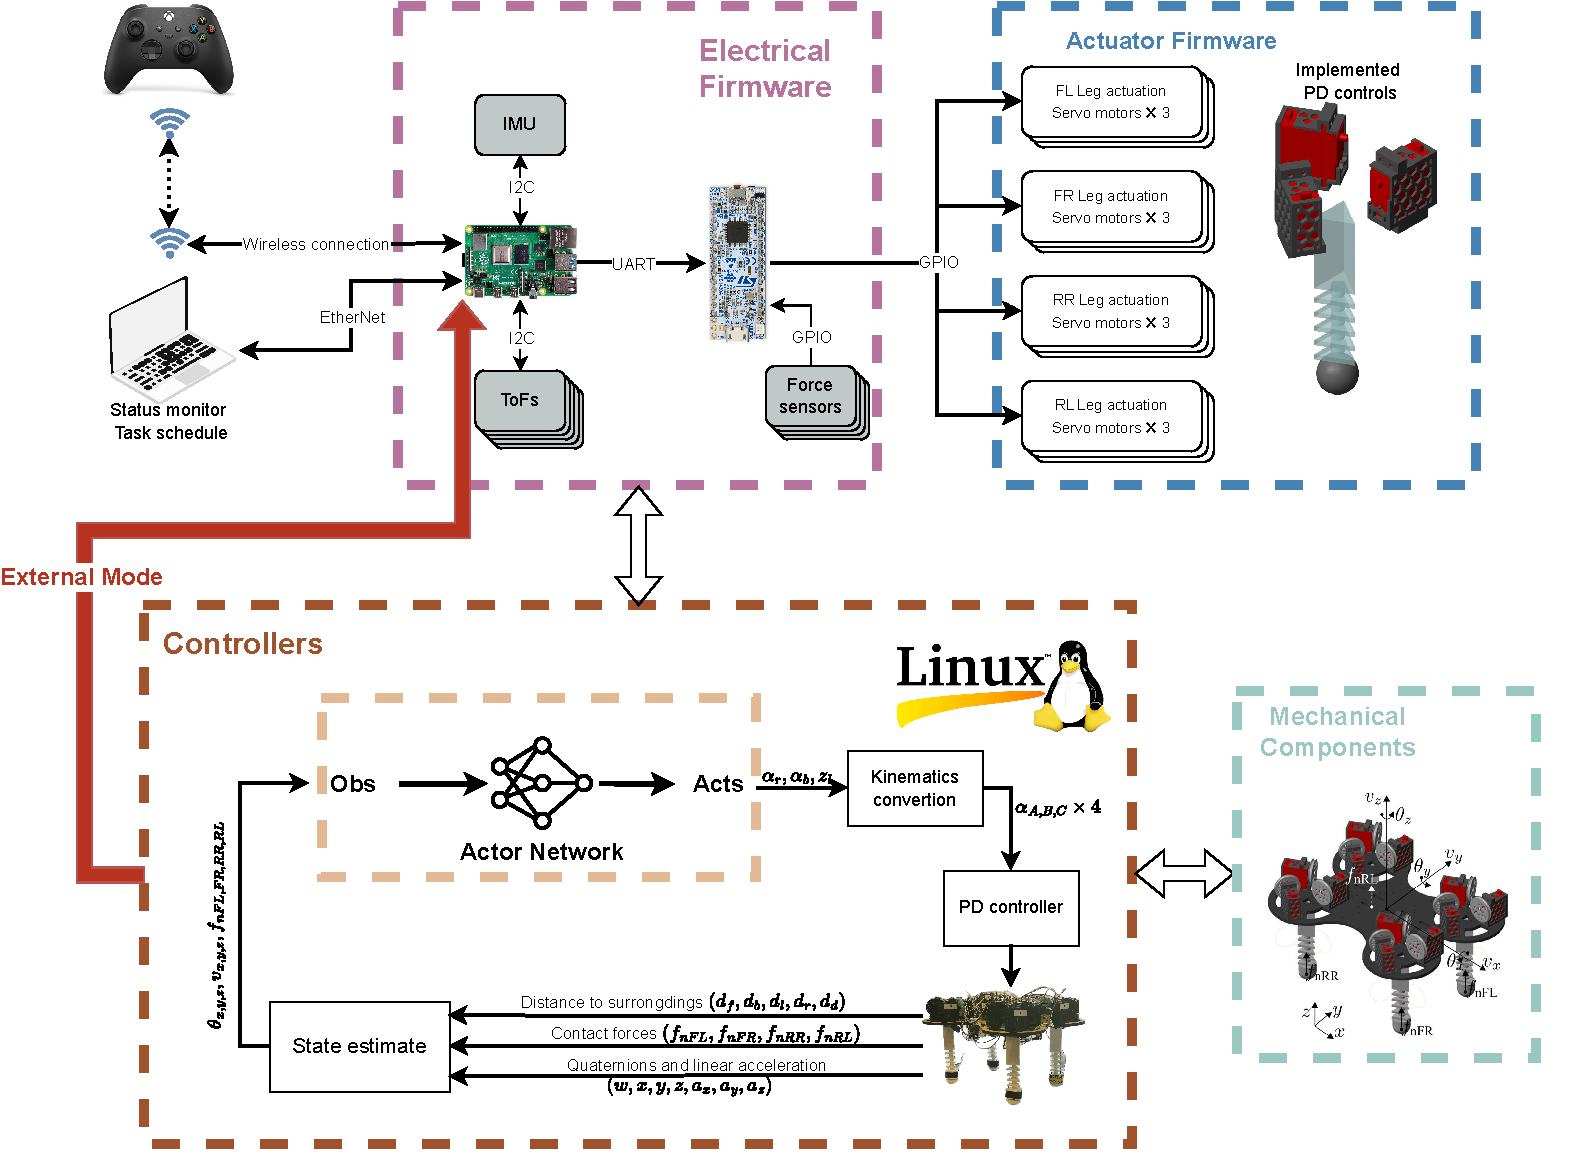
\includegraphics[width=\linewidth]{img/chap4/control.pdf}
    \caption{Graphical overview of control architecture of SoftQ.}
    \label{fig:control}
\end{figure}

The locomotion of SoftQ is profoundly governed by servo motors, which receive \ac{PWM} signals from the STM32 microcontroller. These signals translate into specific rotational torques applied to the actuators, leading to controlled limb motions for different gaits. The servo motors feature built-in position controllers that respond to PWM signals, ensuring precise motor positioning.

The STM32 microcontroller manages contact forces and controls the servo motors through \ac{GPIO} pins. It efficiently processes commands from the Raspberry Pi, generating PWM signals in response to Simulink controller commands. This fine-grained control guarantees accurate execution of the robot's intended actions. Additionally, the STM32 interfaces with force sensors, reading voltage values across them. These voltage changes help the controller determine the applied forces' magnitude, serving as feedback for the robot to adapt its movements to external forces. Communication between the Raspberry Pi and STM32 utilizes \ac{UART} for command and data exchange.

The Raspberry Pi directly interfaces with a variety of sensors and devices to gather supplementary information for guiding the robot's control. These vital observations encompass quaternion angles, linear accelerations, and distance data, all of which are acquired through the \ac{I²C} interface. The quaternion angles, originating from the \ac{IMU}, provide a representation of the robot's orientation in three-dimensional space. For a detailed description of the conversion process from quaternion to Euler angles, please refer to Section \ref{sec:Q2E}. To enhance the situational awareness, these quaternion angles are converted into Euler angles, specifically roll, pitch, and yaw. The IMU itself is a sophisticated 9-DOF sensor, featuring integrated sensor fusion capabilities via its onboard microcontroller. This functionality allows the IMU to provide additional fused data, including linear accelerations in three axis. The linear accelerations is subsequently integrated with distance data from \ac{ToF} sensors to estimate the robot's actual velocity. ToF sensors employ the time-of-flight principle by emitting light pulses that bounce off objects, returning to the sensor to calculate the mean distance within a square area in front of it, measuring the distance between the sensor and the reflecting object.

In the context described, the Simulink controller plays a crucial role by assuming the task of generating the robot's actions through external mode operation on the Raspberry Pi. This entails the generation of control commands, which are determined based on the assessment of states inferred from direct observations. To facilitate this process, raw data such as orientation, linear accelerations, and contact forces of the robot are subjected to preprocessing, transforming them into states ($\mathbf{s}_t$) that can serve as inputs for the actor network. The actor network, which is derived from a converged SAC algorithm, serves as the core component in this control scheme. The actor network takes on the critical task of planning an optimal gait, generating actions that enable the robot to move forward effectively. However, it is essential to note that these actions, produced by the actor network, must undergo a further transformation before they can be effectively utilized by the lower-level controllers. This transformation step involves the conversion of the actions into motor commands. This conversion process relies on inverse kinematic relations, as outlined in Equation \ref{eq:value2motor}. This ensures that the actions generated by the actor network are translated into commands that directly influence the robot's motors, thereby enabling the desired movements and control of the robot's behavior.

Furthermore, the Raspberry Pi establishes wireless communication with a PC to enhance its functionality. The PC serves as a conduit for transferring MATLAB Simulink programs to the Raspberry Pi via external mode. It also acts as a Graphical User Interface (GUI), enabling seamless human-robot interaction. The GUI offers real-time status updates, providing immediate insights into the robot's performance and operation. Moreover, it facilitates the reception of tasks and instructions from the operator, allowing real-time directive issuance. This bidirectional communication between the PC and the robot enhances versatility and adaptability. Additionally, the control system accommodates user input, offering various interfaces like joysticks or command line velocity inputs for real-time robot guidance and adjustments.

\subsection{Task Planning and Execution}
The control architecture of the soft quadruped robot encompasses a multifaceted orchestration of task planning and execution, which plays a pivotal role in the robot's ability to achieve its goals with precision and adaptability. This section delves into the specific architecture of task planning and execution at software side within the control framework. 

The core of the robot's control architecture is centered around the efficient utilization of multi-threading. Each thread is responsible for a specific aspect of the robot's operation, and these threads run concurrently, allowing for parallel processing and efficient resource management. This concurrent execution is particularly advantageous in enhancing the robot's ability to perform multiple tasks simultaneously. Notably, the Raspberry Pi serves as the primary processing unit responsible for coordinating the robot's actions. Within this Raspberry Pi-based control unit, four distinct threads operate in unison to orchestrate the robot's functions: 
\begin{itemize}
    \item UDP\_Transmit Thread (20 Hz): This thread is responsible for reading, composing and transmitting observational data to the Simulink environment via User Datagram Protocol (UDP). It facilitates the seamless exchange of sensory information gathered by the robot with the Simulink simulation. The frequency is bounded by the I²C communication of 5 ToFs. 
    \item UDP\_Receive Thread (50 Hz): The UDP\_Receive thread specializes in receiving motor control commands from the Simulink environment via UDP communication. It ensures that the robot can receive real-time instructions from the simulation, allowing for dynamic control adjustments. Importantly, this thread operates conditionally, only receiving commands when a specific counter condition is met, contributing to safety and controlled execution.
    \item com2STM32 Thread (20 Hz): This thread is responsible for bidirectional communication with the STM32 microcontroller, which interfaces with the robot's hardware components. It sends relevant control data to the STM32 unit, enabling the robot to perform physical actions. Simultaneously, it receives sensor readings and feedback from the STM32, providing crucial information about the robot's state and surroundings. The frequency is bounded by the computation load from Simulink. 
    \item Countdown Thread (0.5 Hz): The Internal Countdown thread operates at a lower frequency of 0.5 Hz. Its primary role is to manage a countdown mechanism that regulates the activation of flags to the STM32, indicating when motor commands received from Simulink can be executed.
\end{itemize}

One fundamental aspect of this architecture is its decentralized nature. Instead of relying on a single central controller, the robot employs a distributed control strategy. Each thread is designed to handle a specific subset of tasks or functionalities. For instance, the STM32 process operates on an event-triggered basis, only executing motor commands when received from the Raspberry Pi. It also sends back contact force readings, adding a feedback loop to the control process. Additionally, the presence of flags controlling the switch of power sources ensures that only reliable motor commands obtained from Simulink are executed, further enhancing the safety and reliability of the robot's actions. 
\begin{figure}[htb]
    \centering
    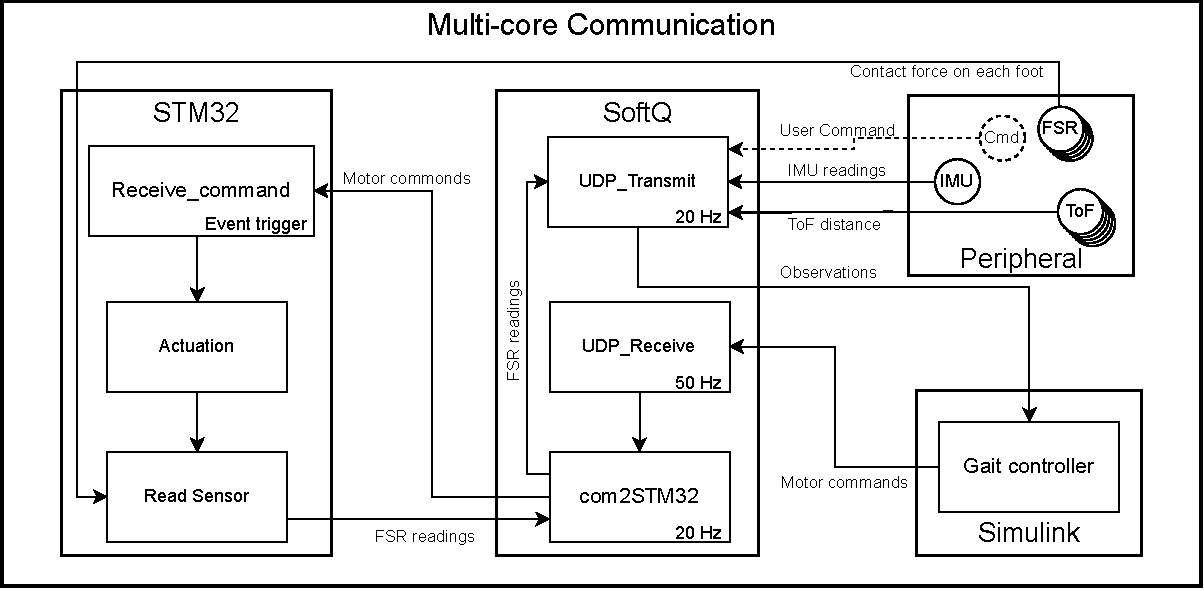
\includegraphics[width=0.9\linewidth]{img/chap4/process.pdf}
    \caption{Schematics of multi-core communication of SoftQ.}
    \label{fig:process}
\end{figure}

To facilitate cooperation among these threads and processes, a well-defined mechanism for multi-core communication and data sharing is established. This mechanism allows threads to exchange information and synchronize their actions. The schematic representation of this multi-core communication is illustrated in Figure \ref{fig:process}. To exemplify this inter-thread communication, consider the SoftQ process running on the Raspberry Pi. Within this context, a "Thread-Safe Data Access" mechanism is meticulously implemented. This involves encapsulating shared data within a dataclass, a structured approach that helps prevent data corruption or conflicts in a multi-threaded environment. Furthermore, synchronization mechanisms such as locks or semaphores are judiciously employed. These synchronization tools serve as safeguards, ensuring that only one thread can access and modify shared data at any given time, thus mitigating the risk of data inconsistency or errors. In addition, the control architecture benefits from pre-designed Direct Memory Access (DMA) and Interrupts Muralidharan et al.\cite{thorapallimuralidharanContinuumActuatorBased2020} and Danelia et al.\cite{daneliaStructureGaitOptimizationof2021}. These advanced techniques enhance data transfer efficiency and response times, further augmenting the control system's capabilities.

\subsection{Sensor Fusion by Kalman Filter}
In this section, the focus shifts to the implementation of a Kalman filter for sensor fusion, a critical element of the research aimed at acquiring precise velocity information. The quest for accurate velocity data is driven by the core objective of achieving precise control and adaptability in the deployment of MBRL on physical robots. Velocity estimation is approached by differentiating the position component over time, with particular attention given to forward walking scenarios, where the angular velocity component can be safely disregarded. The instant velocity calculated based on the distance data from the ToF sensors is plotted in Figure \ref{fig:KF}. However, this velocity exhibits a sharp changes and may not effectively capture dynamic changes in velocity. Furthermore, the computed velocity may result from the integration of linear acceleration over time, as plotted in Figure \ref{fig:KF}. This approach, unfortunately, is susceptible to inaccuracies, with the calculated velocity exhibiting constant fluctuations even in the absence of motion. The source of this inaccuracy is attributed to the drift present in the acceleration data acquired from the IMU. Consequently, the velocity estimation from acceleration reaches a constant value at -0.8 m/s after walk. 
\begin{figure}[htb]
    \centering
    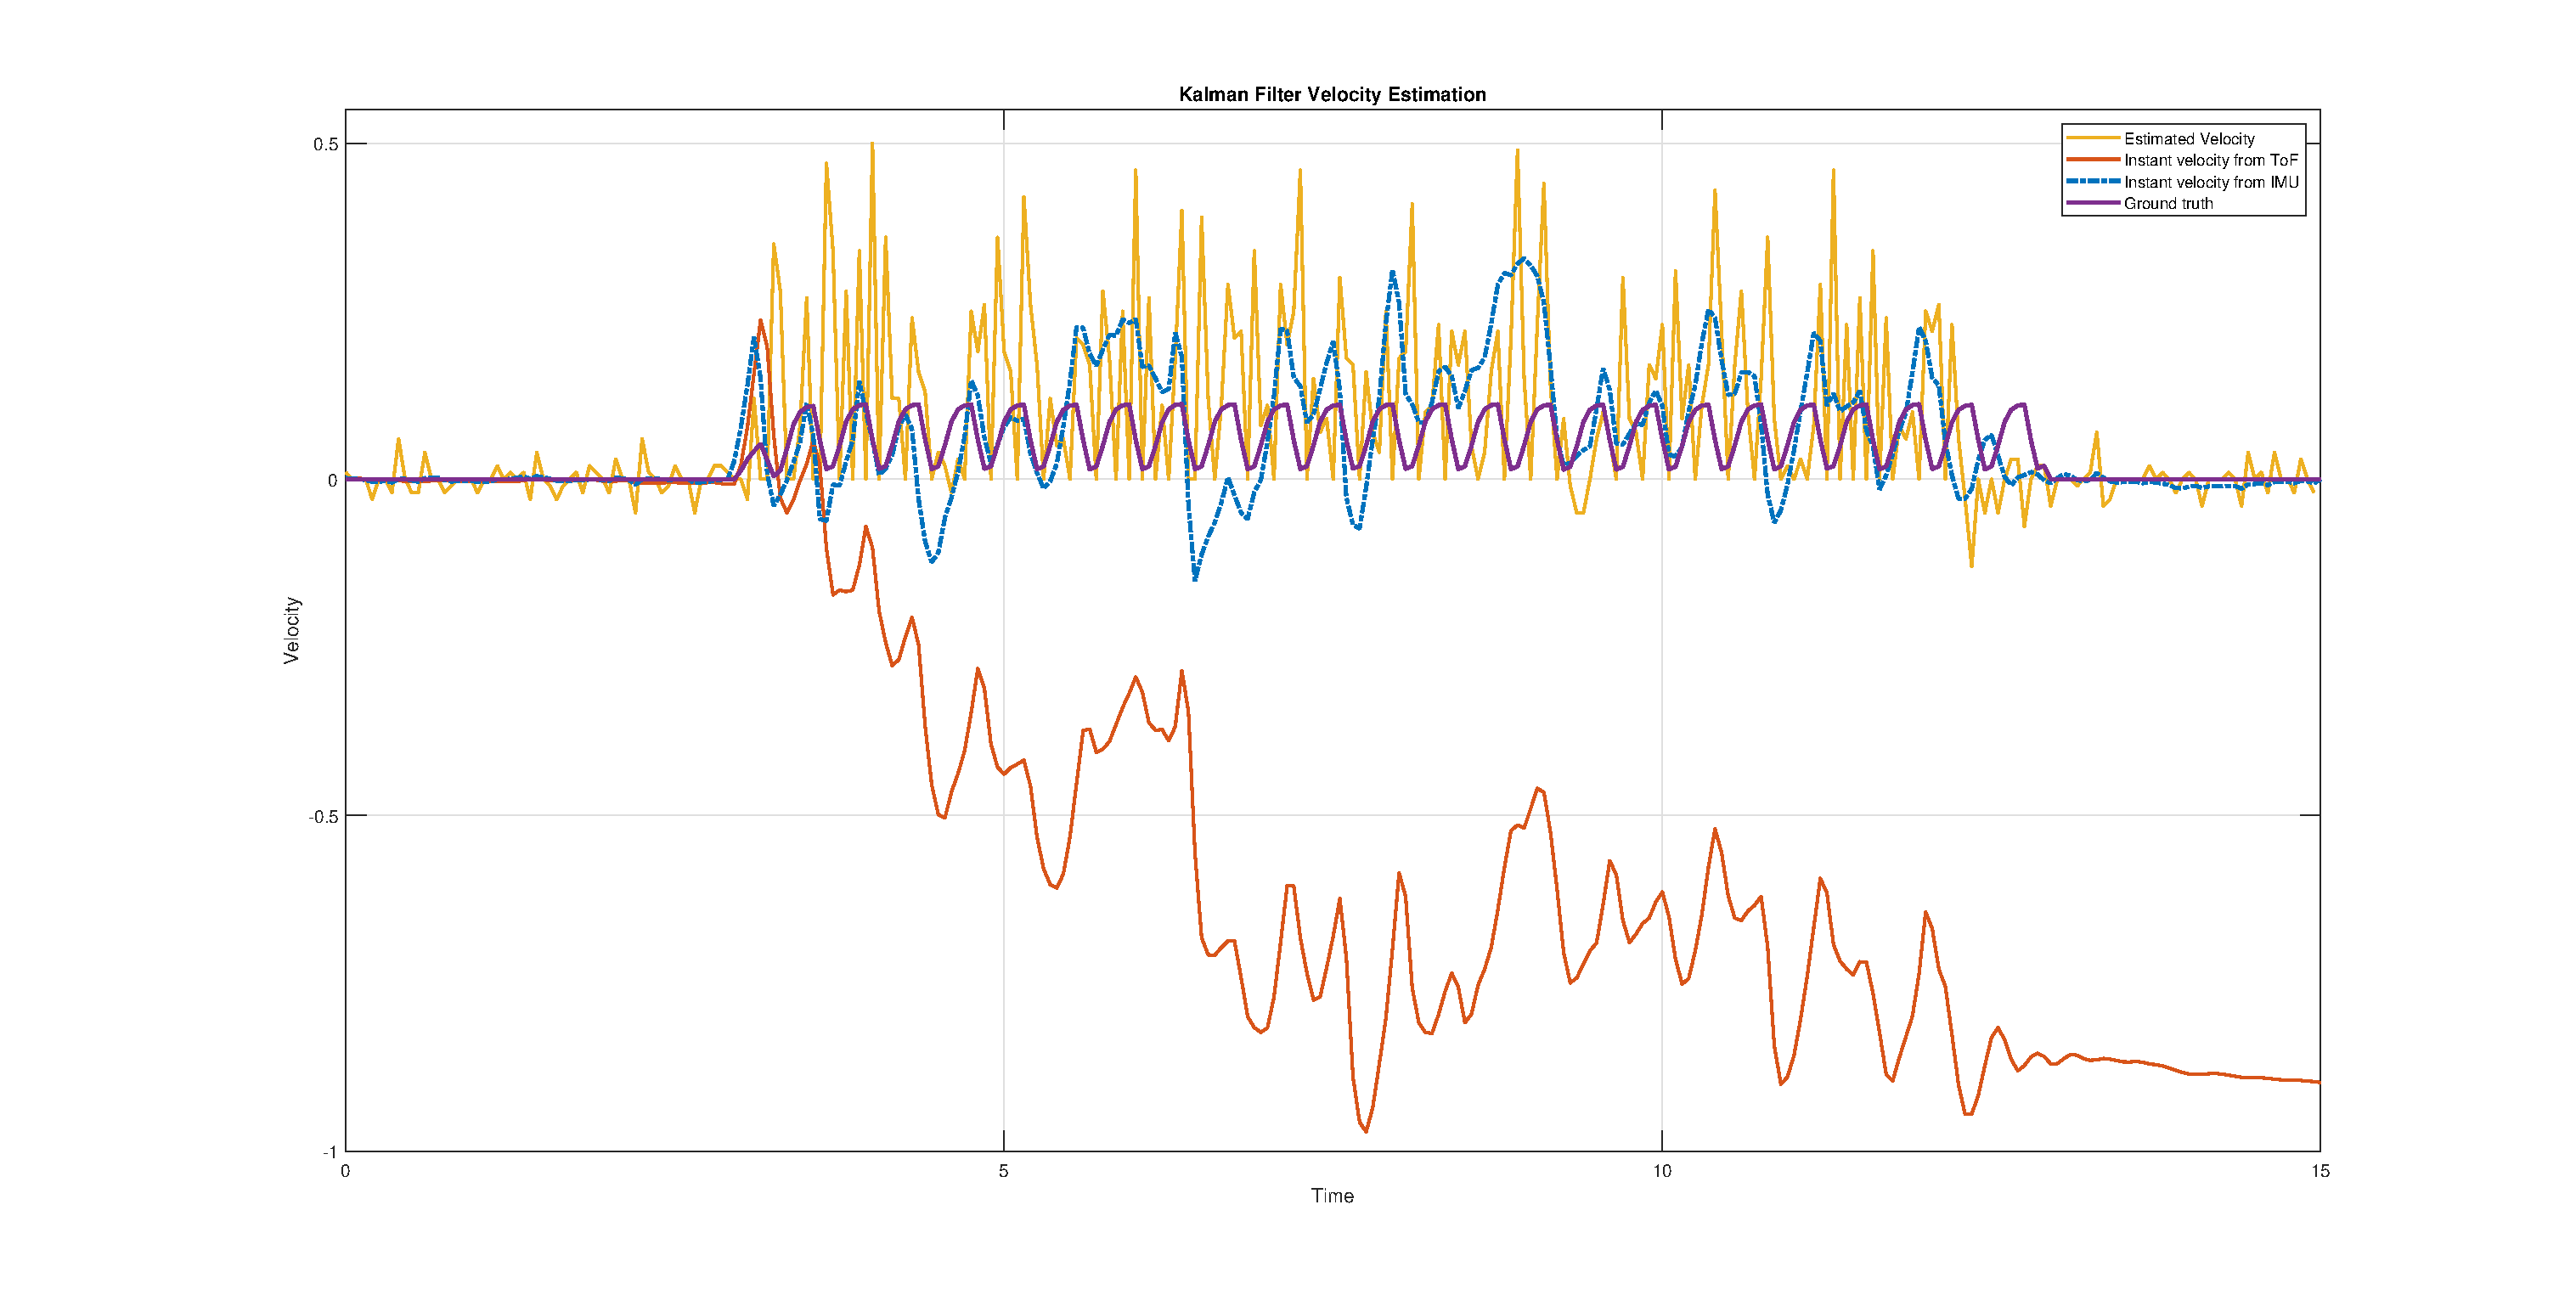
\includegraphics[width=\linewidth]{img/chap4/KF.eps}
    \caption{Velocity estimation in x-axis ($v_x$) through Kalman filtering of ToF and IMU data.}
    \label{fig:KF}
\end{figure}

To achieve a more accurate and precise velocity estimation, a Kalman filter has been specifically designed and integrated into the control architecture. The Kalman filter assumes a crucial role in reducing sensor electronic noise, addressing measurement inaccuracies, mitigating sensor noise, and minimizing quantization errors when predicting velocity from acceleration and position measurements. However, it's important to note that obtaining ground truth velocity data from the real robot is complex. Therefore, we used velocity data from simulations of the tested expert gait as a reference, as shown in Figure \ref{fig:KF}. The Kalman filter's estimation appears to capture most of the movement periods, although some inconsistencies remain. This is attributed to the reality gap, as the robot faces challenges in maintaining a relatively constant speed due to differences in ground conditions and other factors in the real-world environment.

Kalman filter is a linear optimal states estimation method, which is known as one of the most famous Bayesian filter theories. State equation is a linear representation of a state vector $x_{k-1}$, a process noise matrix $w_{k}$ and a control input vector $u_{k}$. Observation equation is a linear representation of a state vector $x_{k}$ and a measurement noise vector $v_{k}$. A dynamic model is presented with state equation and observation equation through the reliable estimation corrected by measurements, which is shown in Equation \ref{eq:kf}.

\begin{equation}
    \begin{aligned}
        \text{State Equation:} \quad & x_{k} = A x_{k-1} + B u_{k-1} + w_{k} \\
        \text{Observation Equation:} \quad & z_{k} = H x_{k} + \nu_{k}
    \end{aligned}
\label{eq:kf}
\end{equation}

In the above formulas: $A$, $H$, $w_{k}$, $\nu_{k}$ is the state transition matrix, the observation matrix, the system noise vector, the observation noise vector, respectively. $w_{k}$ and $\nu_{k}$ are assumed to satisfy positive definite, symmetric and uncorrelated, zero mean Gaussian white noise vector. $w_{k}$ is a random variable with a multivariate normal distribution, where the covariance matrix is $Q$. $\nu_{k}$ is also assumed to be a random variable with a multivariate normal distribution, where the covariance matrix is $R$. In addition, The state covariance matrix, denoted as $P$, is a symmetric matrix that provides information about the uncertainty in the state variables being estimated by the Kalman filter. $P$ undergoes continuous updates as the Kalman filter processes new measurements and predictions. In specific, the Kalman filter is appled to a linear system, and the system dynamics can be approximated as a linear relation between the acceleration $a$, velocity$v$ and position $p$, namely 
\begin{align*}
    \begin{cases} 
    p = p + T_s\cdot v + \frac{T_s^2}{2}\cdot a\\
    v = v + T_s\cdot a
    \end{cases}
    \label{eq:kf_dynamics}
\end{align*}

Defining the states as $x_1 = p$, $x_2 = v$ and the input $u = a$, the model could be transformed into state space form
\begin{equation}
    \begin{cases} 
    \mathbf{x}_{k+1} = \begin{bmatrix}p \\v \end{bmatrix} = \underbrace{\begin{bmatrix}1 & T_s \\0 & 1\end{bmatrix}}_{A} \mathbf{x}_k + \underbrace{\begin{bmatrix}\frac{T_s^2}{2}  \\T_s \end{bmatrix}}_{B} u_k \\
    y_k = \underbrace{\begin{bmatrix}1\;0\end{bmatrix}}_{H} \mathbf{x}_k
    \end{cases}
    \label{eq:kf_state}
\end{equation}

The Kalman gain $K$ determines the weight given to incoming measurement data when updating the estimated state of a dynamic system. In each step, $K_k$ is updated by $P_k$, $K_k=\frac{P_kH}{HP_kH^T+R}$. The Kalman gain $K_k$ emerges as a critical factor in adjusting the state estimate in response to incoming measurements, as outlined in the state estimation equation:
\begin{equation}
    \hat{\mathbf{x}}_{k+1} = A\hat{\mathbf{x}}_{k-1} + Bu_k + K_k\cdot(z_k - H\hat{\mathbf{x}}_{k-1})
    \label{eq:kf_est}
\end{equation} 
In this equations, $\hat{\mathbf{x}}_{k+1}$ is the updated state estimate, $u_k$ is the control input, $z_k$ is the measurement in position. The observer is interpreted as a one-step predictor, which forecasts the system states at the next time instance $k+1$ by utilizing the estimated states at time $k$, along with additional feedback from the estimation error, weighted by the Kalman gains. Since the disturbance primarily affects the acceleration, we can update the structure of $Q$ accordingly. The process noise covariance matrix $Q$ should reflect the covariance of disturbances in acceleration ($\sigma_a^2$) and how they propagate through the system. In a simplified form, it might look like: $Q = \begin{bmatrix}0.01 & 0 \\0 & 1\end{bmatrix}$, and the observation noise covariance matrix is set as $R = 0.15$. Additionally, the observation noise covariance matrix is tuned to be $R = 0.1$, and initial state estimates ($\mathbf{x}_0$) and initial error covariance estimates ($P_0$) are provided as: $\mathbf{x}_0 = \begin{bmatrix} 0 \\ 0 \end{bmatrix}$ and $P_0 = \begin{bmatrix}1 & 0 \\0 & 1\end{bmatrix}$. 

The detailed process of how the Kalman filter is updated and applied can be found in Section \ref{sec:kf}. Before incorporating sensor measurements into the Kalman filter, a preprocessing step was performed to bound and average the measurements, ensuring their reliability and stability. The same Kalman filter for sensor fusion was employed for velocity estimation in both the $x$ and $y$ axes. This choice was driven by the presence of two Time-of-Flight (ToF) sensors dedicated to these axes. Conversely, in the $z$ axis, which represents vertical motion, a single ToF sensor located at the bottom was used. The optimal state observer, known as the Kalman filter provides the optimal estimate of $\mathbf{x}$ minimizing the covariance matrix $P$ of the estimation error $\hat{\mathbf{x}}$ using series of noisy measurements. As the Kalman filter iteratively processed sensor measurements, it progressively refined its estimates of velocity. The results of velocity estimation, facilitated by the Kalman filter application, are visualized and presented in Figure \ref{fig:KF}. These plots provide a clear representation of the refined velocity estimates and underscore the effectiveness of the Kalman filter in mitigating sensor noise and enhancing the overall reliability of the velocity sensing.

\section{Potential Reality Gap}
Transitioning to a different facet of consideration, it's crucial to address the concept of the "Potential Reality Gap." In the realm of reinforcement learning, the surrogate model serves as a bridge between simulation environments and real-world scenarios. However, due to the inherent complexity and uncertainty associated with real-world environments, a misalignment often arises between the training data collected from simulations and the actual performance of the trained model in real-world situations. This discrepancy is referred to as the "Reality Gap."

The Reality Gap poses a challenge because the surrogate model might perform exceptionally well during training in simulation environments but struggle to generalize effectively to real-world settings. This phenomenon can be attributed to various factors, including disparities in physical dynamics, sensor noise, and unmodeled environmental influences. To address the Reality Gap, certain strategies can be adopted. One approach involves introducing stochasticity during training in simulations, simulating uncertainties and disturbances that are characteristic of real-world scenarios, where zero mean Gaussian noise is introduced into all observation signals. This additional noise is independently sampled from zero-mean Gaussian distributions in a random manner. Based on the sensor calibration results, the variances of the noise applied to the velocity, angular and force signal data are set to: $\sigma_{\pmb{\theta}}^2 = 0.002$, $\sigma_{\mathbf{v}}^2 = 0.002$ and $\sigma_{\mathbf{f}_n}^2 = 0.005$, respectively. By incorporating such noise into the training process, the model is better equipped to develop robustness and adaptability, allowing it to effectively handle unexpected variations and challenges encountered in real-world applications.

In an effort to mitigate the Reality Gap, it's worth noting that the SAC algorithm offers commendable exploration capabilities. This presents the opportunity to retrain a converged agent with the potential to adapt its policy for various tasks. Consequently, the converged policy guiding the robot's walking behavior, as determined by MBRL, can be repurposed as the initial policy for continued training with a more accurate model, facilitating the reduction of the Reality Gap, which is so-called continuous training.

The continuous training begins by extracting the policy that has been converged during the initial MBRL training. This policy is the result of the agent's learning process and encapsulates the knowledge it has gained about optimal gait control. To address the reality gap, the converged policy is integrated with a more accurate simulation model in Matlab. This simulation would strive to closely replicate the real-world dynamics and physics of the robot. The use of a more accurate model helps in reducing the discrepancies between simulation and reality. The training process begins with the converged policy as the starting point. This initial policy is influenced by the agent's prior learning, facilitating faster adaptation to the refined simulation environment. Depending on the specific goals and challenges of the new simulation setup, it is important to adjust the reward structure by fine-tuning reward functions to align with desired behavior or objectives in the updated environment. Once the continuous training process has yielded a sufficiently adapted policy, this policy can be transferred to the physical robot for real-world testing. 